%%%%%%%%%%%%%%%%%%%%%%%%%%%%%%%%%%%%%%%%%%%%%%%%%%%%%%%%%%%%%%%%%%%%%%%%%%%%%%%%
% Main TeX file for PhD thesis
%%%%%%%%%%%%%%%%%%%%%%%%%%%%%%%%%%%%%%%%%%%%%%%%%%%%%%%%%%%%%%%%%%%%%%%%%%%%%%%%


%%%%%%%%%%%%%%%%%%%%%%%%%%%%%%%%%%%%%%%%%%%%%%%%%%%%%%%%%%%%%%%%%%%%%%%%%%%%%%%%
% Formatting and package includes
%%%%%%%%%%%%%%%%%%%%%%%%%%%%%%%%%%%%%%%%%%%%%%%%%%%%%%%%%%%%%%%%%%%%%%%%%%%%%%%%
\documentclass[12pt,a4paper,twoside]{book}
%--------------------------------------------------------------------------------
% Make figures stick to the top of the page, when there is no text.
% For example, on the last page of a chapter.
%--------------------------------------------------------------------------------
\makeatletter
\setlength{\@fptop}{0pt}
\makeatother
\PassOptionsToPackage{english}{babel}
%%%%%%%%%%%%%%%%%%%%%%%%%%%%%%%%%%%%%%%%%%%%%%%%%%%%%%%%%%%%%%%%%%%%%%%%%%%%%%%%
% Thesis formatting style
%%%%%%%%%%%%%%%%%%%%%%%%%%%%%%%%%%%%%%%%%%%%%%%%%%%%%%%%%%%%%%%%%%%%%%%%%%%%%%%%


%--------------------------------------------------------------------------------
% Packages
%--------------------------------------------------------------------------------
\usepackage{times}

\usepackage{color}				% Allow colored text
\usepackage{graphicx}			% Allow graphics

\usepackage{fancyhdr}			% Custom headers
\usepackage{enumerate}			% Custom enum
\usepackage{cite}				% otherwise citations are not set nicely

\usepackage{algorithm}
\usepackage{algorithmic}
\usepackage{subfigure}
\usepackage{amsmath}
\usepackage{amssymb}

\usepackage{tabularx}
\usepackage{array}
\usepackage{CV}


%--------------------------------------------------------------------------------
% Define colors
%--------------------------------------------------------------------------------
\definecolor{RED}{RGB}{255,0,0}
\definecolor{GREEN}{RGB}{0,255,0}
\definecolor{BLUE}{RGB}{0,0,255}
\definecolor{GRAY}{RGB}{128,128,128}
\definecolor{BLACK}{RGB}{0,0,0}


%--------------------------------------------------------------------------------
% Useful Commands
%--------------------------------------------------------------------------------
\newcommand{\RENATO}[1]{\textbf{\color{RED}{RENATO: #1}}}
\newcommand{\FATIH}[1]{\textbf{\color{GREEN}{FATIH: #1}}}

\newcommand{\itemtitle}[1]{\addtolength{\parskip}{3mm}{\noindent\bf {#1}} \addtolength{\parskip}{-3mm}}

% Define degree command
\newcommand{\degree}{\ensuremath{^\circ}}


%--------------------------------------------------------------------------------
% Book layout
%--------------------------------------------------------------------------------
\input{letterspacing.tex} % define the spacing between letters -> used for the word chapter
\usepackage[nottoc]{tocbibind} % used to include bibliography in the table of contents

% PDF bookmarks
% \usepackage[bookmarks=true,bookmarksnumbered=true]{hyperref}

\usepackage{xspace}

\hyphenation{Leap-frog}


% Manually set margins, so that the bigger space is on correct side
\setlength\oddsidemargin{0.7in}
\setlength\evensidemargin{0.14in}


%--------------------------------------------------------------------------------
% Headers and Footers
%--------------------------------------------------------------------------------
\pagestyle{fancy}
\fancyhf{}

\renewcommand{\chaptermark}[1]{%
\markboth{\MakeUppercase{\thechapter \space \ #1}}{}}

\renewcommand{\sectionmark}[1]{\markright{\thesection \space\ #1}}

\fancyhead[LE,RO]{\footnotesize\usefont{T1}{fvs}{n}{n}\selectfont\thepage}
\fancyhead[RE]{\footnotesize \usefont{T1}{fvs}{n}{n}\selectfont{\leftmark}}
\fancyhead[LO]{\footnotesize\usefont{T1}{fvs}{n}{n}\selectfont{\rightmark}}
\headsep 1cm % abstand header - text

% Chapters have to start on an odd page. So, if the chapter before ended on odd page, there is an empty page
% inbetween, which still gets header and footer that looks bad. We redefine how LaTeX adds the empty page.
\makeatletter
\def\cleardoublepage{\clearpage\if@twoside \ifodd\c@page\else
\hbox{}
\thispagestyle{empty}
\newpage
\if@twocolumn\hbox{}\newpage\fi\fi\fi}
\makeatother


%--------------------------------------------------------------------------------
% Section titles
%--------------------------------------------------------------------------------
\usepackage{sectsty}
\allsectionsfont{\large \usefont{T1}{fvs}{b}{n}\selectfont}
\subsectionfont{\normalsize \usefont{T1}{fvs}{b}{n}\selectfont}
\subsubsectionfont{\small \usefont{T1}{fvs}{b}{n}\selectfont}
\paragraphfont{\small \usefont{T1}{fvs}{b}{n}\selectfont}


%--------------------------------------------------------------------------------
% Chapter titles
%--------------------------------------------------------------------------------
\definecolor{NUMCOLOR}{rgb}{0.22,0.37,0.56}

\usepackage{multirow} % for tables with multiple rows

% The first makeatletter is to define the chapter layout in the real "Chapter" chapters
\makeatletter
\def\@makechapterhead#1{%
 % \vspace*{10\p@}%
  %\hrule

  \line(1,0){0}
  \newline
  {
  	 %\begin{tabular}{|@{}l|r@{}@{}|}
	 \begin{tabular}{@{}lr@{}@{}}
	 %\hline
	 \linethickness{ 4px }\color{NUMCOLOR}\line(1,0){245}
	& \multirow{2}{*}{\fontsize{100}{62}\usefont{OT1}{ptm}{m}{n}\selectfont \color{NUMCOLOR} \thechapter}\\ % ptm
	 & \\
	% \Huge \bfseries \usefont{OT1}{phv}{m}{n}\selectfont \scshape\@chapapp \hspace{8.25cm} & \\
	%\scshape \bfseries\Huge \@chapapp \hspace{8.25cm}
	\scshape \LARGE \usefont{T1}{fvs}{sc}{n}\selectfont \letterspace to 2.5\naturalwidth{CHAPTER} \hspace{3cm}
	& \\
	%\hline
	\end{tabular}

\vskip 100\p@
\raggedleft
    \interlinepenalty\@M
    \scshape \fontsize{24}{30} \usefont{T1}{fvs}{n}{n}\selectfont \scshape \MakeUppercase{#1}\par\nobreak
      \vskip 80\p@%60
  }
  }


% The second makeatletter is to define the chapter layout in the chapters like Abstract etc. (almost identical but without the word "chapter" and some ugly hacks which are necessary to align the titles)
\makeatletter
\def\@makeschapterhead#1{%
 % \vspace*{10\p@}%
  %\hrule

  \line(1,0){0}
  \newline
  {
  	 %\begin{tabular}{|@{}l|r@{}@{}|}
	 \begin{tabular}{@{}lr@{}@{}}
	 %\hline
	 \linethickness{ 4px }\color{NUMCOLOR}\line(1,0){245}
	& %\multirow{2}{*}{\fontsize{100}{62}\usefont{OT1}{ptm}{m}{n}\selectfont \color{NUMCOLOR} \thechapter}
	\\ % ptm
	 & \\
	% **HACK** add vspace.
	% otherwise these titles and the chapter titles are not at the same place
	% because the word "chapter" is missing and latex rearranges everything, no clue why
	% vspace value is manually tuned
	\scshape \LARGE \usefont{T1}{fvs}{sc}{n}\selectfont \letterspace to 2.5\naturalwidth{} \hspace{3cm} \vspace{0.17cm}
	& \\
	%\hline
	\end{tabular}

\vskip 100\p@
\raggedleft
    \interlinepenalty\@M
    \scshape \fontsize{24}{30} \usefont{T1}{fvs}{n}{n}\selectfont \scshape \MakeUppercase{#1}\par\nobreak
      \vskip 80\p@
  }
  }


%--------------------------------------------------------------------------------
% Table of Contents font
%--------------------------------------------------------------------------------
\usepackage[titles]{styles/tocloft}
\renewcommand{\cftchapfont}{\fontsize{11}{13}\usefont{T1}{fvs}{b}{n}\selectfont}


%--------------------------------------------------------------------------------
% Figure captions
%--------------------------------------------------------------------------------
\usepackage[font=small,format=plain,labelfont=bf,up,textfont=it,up]{caption}


%--------------------------------------------------------------------------------
% Notation list
%--------------------------------------------------------------------------------
\usepackage[intoc]{nomencl}
\usepackage{ifthen}

% Change title
\renewcommand{\nomname}{Notations}
\setlength{\nomlabelwidth}{.25\hsize}       %Aufteilung der Seite
% Define subgroups
\renewcommand{\nomgroup}[1]
{
	\ifthenelse{\equal{#1}{A}}
	{\item[\fontsize{11}{13}\usefont{T1}{fvs}{b}{n}\selectfont{Acronyms}]}
 	{
	\vspace{1cm} % Abstand zwischen den einzelnen Bl�cken

	\ifthenelse{\equal{#1}{B}}
	{\item[\fontsize{11}{13}\usefont{T1}{fvs}{b}{n}\selectfont{Operators and Functions}]}
	{

	\ifthenelse{\equal{#1}{C}}
	{\item[\fontsize{11}{13}\usefont{T1}{fvs}{b}{n}\selectfont{Physics}]}
	{

	\ifthenelse{\equal{#1}{D}}
	{\item[\fontsize{11}{13}\usefont{T1}{fvs}{b}{n}\selectfont{Fluid Particles}]}
	{

	\ifthenelse{\equal{#1}{E}}
 	{\item[\fontsize{11}{13}\usefont{T1}{fvs}{b}{n}\selectfont{Solid Particles}]}
 	{

	\ifthenelse{\equal{#1}{F}}
	{\item[\fontsize{11}{13}\usefont{T1}{fvs}{b}{n}\selectfont{Surface Points}]}
	{
		{}
	}
	}
	}
	}
	}
	}

	\item[]\hspace*{-\leftmargin}%
	\rule[2pt]{1\textwidth}{1pt}%
}


%--------------------------------------------------------------------------------
% Other
%--------------------------------------------------------------------------------
% Decrease row spacings
\setlength{\nomitemsep}{-\parsep}

% Make nomenclature
\makenomenclature

% Image-Text spacing
\floatsep30pt
\textfloatsep 35pt

%%%%%%%%%%%%%%%%%%%%%%%%%%%%%%%%%%%%%%%%%%%%%%%%%%%%%%%%%%%%%%%%%%%%%%%%%%%%%%%%
% Mathematical syntax
%%%%%%%%%%%%%%%%%%%%%%%%%%%%%%%%%%%%%%%%%%%%%%%%%%%%%%%%%%%%%%%%%%%%%%%%%%%%%%%%


%--------------------------------------------------------------------------------
% Commands
%--------------------------------------------------------------------------------
\newcommand{\Adjoint}{\mbox{\rm Adj}}
\newcommand{\Area}{\mbox{\rm Area}}
\newcommand{\ACos}{{\mbox{\rm Cos}^{-1}}}
\newcommand{\ASin}{{\mbox{\rm Sin}^{-1}}}
\newcommand{\ATan}{{\mbox{\rm atan2}}}
\newcommand{\Code}[1]{{\tt #1}}
\newcommand{\Complex}{\mbox{\bf C}}
\newcommand{\Cross}{{\mbox{\rm Cross}}}
\newcommand{\Mydddot}[1]{\mbox{\shortstack{$.$\hspace*{-1pt}$.$\hspace*{-1pt}$.$\\$#1$}}}
\newcommand{\Degree}{\mbox{\rm degree}}
\newcommand{\Diag}{\mbox{\rm Diag}}
\newcommand{\Dim}{\mbox{\rm dim}}
\newcommand{\Dist}{\mbox{\rm Distance}}
\newcommand{\IntTwo}{\int\!\!\int}
\newcommand{\IntThree}{\int\!\!\int\! \!\int}
\newcommand{\Kernel}{\mbox{\rm kernel}}
\newcommand{\Kross}{\mbox{\rm Kross}}
\newcommand{\Grad}{\nabla}
\newcommand{\Perp}{\mbox{\rm Perp}}
\newcommand{\Point}[1]{{\cal #1}}
\newcommand{\Rank}{\mbox{\rm rank}}
\newcommand{\Range}{\mbox{\rm range}}
\newcommand{\Real}{{\mbox{\rm I}\hspace*{-2pt}\mbox{\rm R}}}
\newcommand{\RealSbt}{{\mbox{\rm\scriptsize I}\hspace*{-2pt}\mbox{\rm\scriptsize R}}}
\newcommand{\Res}{\mbox{\rm resultant}}
\newcommand{\Sbt}[1]{{\mbox{\rm\scriptsize #1}}}
\newcommand{\MySign}{\mbox{\rm Sign}}
\newcommand{\SignSBT}{\mbox{\rm\scriptsize Sign}}
\newcommand{\Skew}{\mbox{\rm Skew}}
\newcommand{\Span}{\mbox{\rm Span}}
\newcommand{\SqrDist}{\mbox{\rm Distance$^2$}}
\newcommand{\Trace}{\mbox{\rm Trace}}
\newcommand{\TRN}{{\mbox{\rm\scriptsize T}}}
\newcommand{\Vector}[1]{\mbox{\bf #1}}
\newcommand{\VectorM}[1]{\mbox{\boldmath $#1$}}
\newcommand{\Volume}{\mbox{\rm Volume}}

\newcommand{\IVec}{\mbox{\boldmath $\imath$}}
\newcommand{\JVec}{\mbox{\boldmath $\jmath$}}
\newcommand{\KVec}{\mbox{\boldmath $k$}}
\newcommand{\LVec}{\mbox{\boldmath $\ell$}}
\newcommand{\RMat}{{\cal R}}
\newcommand{\QMat}{{\cal Q}}
\newcommand{\QCMat}{\overline{\cal Q}}

\newcommand{\Lerp}{\mbox{\rm lerp}}
\newcommand{\Slerp}{\mbox{\rm slerp}}
\newcommand{\Quad}{\mbox{\rm quad}}
\newcommand{\Squad}{\mbox{\rm squad}}

\newcommand{\ODer}[2]{\frac{d #1}{d #2}}
\newcommand{\ODerT}[2]{\frac{d^2 #1}{d {#2}^2}}
\newcommand{\ODerM}[3]{\frac{d #1}{d #2 \, d #3}}
\newcommand{\PDer}[2]{\frac{\partial #1}{\partial #2}}
\newcommand{\PDerT}[2]{\frac{\partial^2 #1}{\partial {#2}^2}}
\newcommand{\PDerM}[3]{\frac{\partial^2 #1}{\partial #2 \, \partial #3}}

% Mass density symbol
\newcommand{\Den}{\delta}


%--------------------------------------------------------------------------------
% Environments
%--------------------------------------------------------------------------------
\newenvironment{BArray}[1]{\left\{ \begin{array}{#1}}{\end{array} \right\}}
\newenvironment{Combin}{\left( \begin{array}{c}}{\end{array} \right)}
\newenvironment{Matrix}[1]{\left[ \begin{array}{#1}}{\end{array} \right]}

\let\mbf=\mathbf
\let\mvec=\mathbf
\let\mcal=\mathcal
\let\mfunc=\mathrm

%\def\R{\mbox{\ensuremath{\mathrm{I\!R}}}}
%\newcommand{\R}{\ensuremath{\mathbb{R}}}
%\newcommand{\N}{\ensuremath{\mathbb{N}}}
%\newcommand{\Z}{\ensuremath{\mathbb{Z}}}
%\newcommand{\C}{\ensuremath{\mathbb{C}}}

\newcommand{\of}[1]{\left( #1 \right)}
\newcommand{\abs}[1]{\left| #1 \right|}
\newcommand{\norm}[1]{\left\Vert {#1} \right\Vert}
\newcommand{\gradient}[1]{\nabla{\!}_{#1}{\,}}
\newcommand{\twovec}[2]{\left( #1 \atop #2 \right)}
\newcommand{\threevec}[3]{\left(\begin{array}{c}#1\\#2\\#3\end{array}\right)}
\newcommand{\fourvec}[4]{\left(\begin{array}{c}#1\\#2\\#3\\#4\end{array}\right)}

\newcommand{\refsec}[1]{Section~\ref{sec:#1}}
\newcommand{\reffig}[1]{Fig.~\ref{fig:#1}}
\newcommand{\reftab}[1]{Tab.~\ref{tab:#1}}
\newcommand{\refeq}[1]{Eq.~(\ref{eq:#1})}

%\newcommand{\R}{\hspace*{0.1ex}{\sf I} \hspace{-0.3ex}{\sf R}}

%6.5
\newcommand{\eps}{\mbox{$\epsilon$}}
\newcommand{\dmin}{\mbox{$d_{\min}$}}
\newcommand{\dmax}{\mbox{$d_{\max}$}}
\newcommand{\dminmax}{\mbox{$[\dmin,\dmax]$}}

%4.2:
\def\M{\mathcal{M}}
\def\n{\mathbf{n}}
\def\p{\mathbf{p}}
\def\q{\mathbf{q}}
\def\x{\mathbf{x}}
\def\tp{^{\mathsf{T}}}

\let\vec=\mathbf%
\let\mat=\mathbf%
\let\set= \mathcal%
\newcommand{\R}{\ensuremath{\mathbb{R}}}
\newcommand{\N}{\ensuremath{\mathbb{N}}}


\usepackage{pbox}
\usepackage{tabularx}
\usepackage{wrapfig}
\usepackage{newfloat}
\usepackage{csvsimple}
\usepackage{paralist}
\usepackage{multibib}
\usepackage{csquotes}
\usepackage{styles/myapalike}
\usepackage{caption}
\usepackage{latexsym}

\definecolor{red}{rgb}{1,0,0}
\newcommand{\fix}[1]{\textbf{\color{red}{#1}}}
\newcommand{\fig}[1]{Figure~\ref{#1}}
\newcommand{\bench}[1]{Benchmark~\ref{#1}}
\newcommand{\cref}[1]{Chapter~\ref{#1}}
\newcommand{\sref}[1]{Section~\ref{#1}}
\newcommand{\aref}[1]{Appendix~\ref{#1}}
\clubpenalty=10000
\widowpenalty=10000
\def\quad{\hspace*{1em}}
\def\qquad{\hspace*{2em}}
\hyphenation{Chro-mium cul-ling}

\DeclareFloatingEnvironment[
  fileext=lor,
  listname={List of Benchmarks},
  name=Benchmark,
  placement=tp,
  %within=section,% activate it if you want
  %chapterlistsgaps=on,% only meaningful when chapters exist
]{benchmark}

\newcites{conf}{Conference Publications}
\newcites{journal}{Journal Articles}

%%%%%%%%%%%%%%%%%%%%%%%%%%%%%%%%%%%%%%%%%%%%%%%%%%%%%%%%%%%%%%%%%%%%%%%%%%%%%%%%
% Document body
%%%%%%%%%%%%%%%%%%%%%%%%%%%%%%%%%%%%%%%%%%%%%%%%%%%%%%%%%%%%%%%%%%%%%%%%%%%%%%%%
\begin{document}
\thispagestyle{empty}
\setcounter{tocdepth}{2}

%%%%%%%%%%%%%%%%%%%%%%%%%%%%%%%%%%%%%%%%%%%%%%%%%%%%%%%%%%%%%%%%%%%%%%%%%%%%%%%%
% Title page 0
%%%%%%%%%%%%%%%%%%%%%%%%%%%%%%%%%%%%%%%%%%%%%%%%%%%%%%%%%%%%%%%%%%%%%%%%%%%%%%%%


\begin{titlepage}

\setlength{\parindent}{0pt} % kein text einzug


\includegraphics[width=6cm]{front/images/uzhlogo.pdf}

\vspace{-2.25cm}

\begingroup
\leftskip7cm

\vspace{-0.75cm}
\Large
\textbf{Parallel Rendering and\\Large Data Visualization}

\vspace{0.70cm}

\normalsize
A dissertation submitted to the Faculty of Economics,
Business Administration and Information Technology of the\\ University of Z\"urich\\

\vspace{0.70cm}

for the degree of\\
Doctor of Science (Ph. D.)

\vspace{0.70cm}

by\\
Stefan Eilemann

\vspace{3.7cm}

Accepted on the recommendation of \\
\\
Prof. Dr. Renato Pajarola\\
Prof. Dr. Markus Hadwiger

\vspace{2.2cm}
\today

\vspace{2.2cm}

\endgroup

\end{titlepage}

%%%%%%%%%%%%%%%%%%%%%%%%%%%%%%%%%%%%%%%%%%%%%%%%%%%%%%%%%%%%%%%%%%%%%%%%%%%%%%%%
% Title page 1
%%%%%%%%%%%%%%%%%%%%%%%%%%%%%%%%%%%%%%%%%%%%%%%%%%%%%%%%%%%%%%%%%%%%%%%%%%%%%%%%


\begin{titlepage}

\setlength{\parindent}{0pt} % kein text einzug

\normalsize
%\fontsize{10}{13}
%\usefont{T1}{fvs}{m}{n}\selectfont
The Faculty of Economics, Business Administration and Information Technology of the University of Zurich herewith permits the publication of the aforementioned dissertation without expressing any opinion on the views contained therein.

\vspace{1cm}
Zurich, \today

\vspace{2cm}
The head of the Ph. D. program in Informatics: Prof. Dr. Sven Seuken
%
\newpage
\thispagestyle{empty}
\quad
\newpage
\setcounter{page}{1}

\end{titlepage}


\pagenumbering{roman}
%%%%%%%%%%%%%%%%%%%%%%%%%%%%%%%%%%%%%%%%%%%%%%%%%%%%%%%%%%%%%%%%%%%%%%%%%%%%%%%%
% Abstract - English
%%%%%%%%%%%%%%%%%%%%%%%%%%%%%%%%%%%%%%%%%%%%%%%%%%%%%%%%%%%%%%%%%%%%%%%%%%%%%%%%


%--------------------------------------------------------------------------------
\chapter*{Abstract}
\addcontentsline{toc}{chapter}{Abstract}
%--------------------------------------------------------------------------------
We are living in the big data age: An ever increasing amount of data is being
produced by users through data acquisition and simulations. While large scale
analysis and simulatons have received significant attention for cloud computing
and HPC systems, software to efficiently visualize large amounts of data is
struggling to keep up.

Large-scale visualization setups are becoming ever more affordable.
High-resolution tiled display walls are in reach even for small institutions,
and can often be driven by a single multi-GPU workstation. Virtual reality has
arrived in the consumer space, driving hardware prices down.

This thesis advances the field of parallel rendering by formalizing the design
and implementation of system software for large data visualization through
parallel rendering, novel algorithms to accelerate the rendering of large
amounts of data, and validates the research and development with new
applications for large data visualization.

Our research and development enables domain scientists and large data
engineers to better extract meaning from their data, making it feasible to
explore more data by accelerating the rendering and allowing the use of
high-resolution displays to see more detail.


%%%%%%%%%%%%%%%%%%%%%%%%%%%%%%%%%%%%%%%%%%%%%%%%%%%%%%%%%%%%%%%%%%%%%%%%%%%%%%%%
% Abstract - German
%%%%%%%%%%%%%%%%%%%%%%%%%%%%%%%%%%%%%%%%%%%%%%%%%%%%%%%%%%%%%%%%%%%%%%%%%%%%%%%%

\chapter*{Kurzfassung}
\addcontentsline{toc}{chapter}{Kurzfassung}

Daten sind das Gold des 21. Jahrhunderts: Computersimulationen, bildgebende
Verfahren und andere Datenerfassungssysteme generieren immer gr\"ossere
Datenmengen. Visualisierungssoftware zur Darstellung grosser Datenmengen ist,
relativ zu Simulationssoftware und verteilten Systemen f\"ur Cloudumgebungen,
in der Forschung und Entwicklung vernachl\"assigt.

Visualisierung ist ein effizientes Mittel um grosse Datenmengen zu analysieren.
Insbesondere die Visualisierung von dreidimensionalen Datens\"atzen erlaubt ein
intuitives Verst\"andnis der r\"aumlichen Zusammenh\"ange und ihrer Struktur.
Visualisierungshardware steht immer mehr Benutzern zur Verf\"ugung,
insbesondere hochaufl\"osende Monitorw\"ande sind mittlerweile auch f\"ur
kleine Institutionen erschwinglich.

Diese Doktorarbeit besch\"aftigt sich mit paralleler Software und Algorithmen
zur Visualisierung dreidimensionaler Datens\"atze, um diesen Entwicklungen
Folge zu tragen. Als Grundlage f\"ur Forschung und Entwicklung formalisieren
wir die Softwarearchitektur f\"ur paralleles Rendering und stellen unsere
Referenzimplementierung vor. Auf dieser Basis pr\"asentieren wir neue
Forschungsergebnisse und Algorithmen zur schnelleren Visualisierung grosser
Datenmengen. Visualisierungssoftware, welche mit unserer Bibliothek entwickelt
wurde, validiert unseren Ansatz, und erlaubt Benutzern mehr Daten mit besserer
Detail zu analysieren.


%%%%%%%%%%%%%%%%%%%%%%%%%%%%%%%%%%%%%%%%%%%%%%%%%%%%%%%%%%%%%%%%%%%%%%%%%%%%%%%%
% Acknowledgments
%%%%%%%%%%%%%%%%%%%%%%%%%%%%%%%%%%%%%%%%%%%%%%%%%%%%%%%%%%%%%%%%%%%%%%%%%%%%%%%%


%--------------------------------------------------------------------------------
\chapter*{Acknowledgments}
\addcontentsline{toc}{chapter}{Acknowledgments}
%--------------------------------------------------------------------------------
The research leading to this proposal was supported in part by the Blue Brain
Project, the Swiss National Science Foundation under Grant 200020-129525, the
European Union Seventh Framework Programme (FP7/2007-2013) under grant agreement
no. 604102 (Human Brain Project), the Hasler Stiftung grant (project number
$12097$), and the King Abdullah University of Science and Technology (KAUST)
through the KAUST-EPFL alliance for Neuro-Inspired High Performance Computing.

I would like to take the opportunity to thank the Blue Brain Project and its
visualization team, RTT AG (now part of Dassault Systems), KAUST, University of
Siegen, the Electronic Visualization Laboratory at the University of Illinois
Chicago, and all the other contributors for their support in the research and
development leading to this thesis.

I would like to thank Prof. Renato Pajarola and the VMML for his long-term
commitment to my research work and Patrick Bouchaud for putting me onto the
path taken by this thesis. Last, but not least, I'ld like to thank all
collaborators who worked with me on this endavour: Daniel Nachbaur, Cedric
Stalder, Maxim Makhinya, Dardo D. Kleiner, Carsten Rohn, Daniel Pfeifer, Sarah
Amsellem, Juan Hernando , Marwan Abdellah, Raphael Dumusc, Lucas Peetz Dulley,
Jafet Villafranca, Philippe Robert, Ahmet Bilgili, Tobias Wolf, Dustin Wueest,
and Martin Lambers.


\tableofcontents
\newpage


% LATEX BUG: chapters of type chapter* following the table of contents show always the table of contents header.
% Workaround: change header manually
\markboth{NOTATIONS}{}

% unix command to update notations list: makeindex thesis.nlo -s nomencl.ist -o thesis.nls
% (set in latex, then makeindex, then set again in latex)
% nomenclature groups are defined in format/styles/thesis.sty
%%%%%%%%%%%%%%%%%%%%%%%%%%%%%%%%%%%%%%%%%%%%%%%%%%%%%%%%%%%%%%%%%%%%%%%%%%%%%%%%
% Nomenclature
%%%%%%%%%%%%%%%%%%%%%%%%%%%%%%%%%%%%%%%%%%%%%%%%%%%%%%%%%%%%%%%%%%%%%%%%%%%%%%%%


\nomenclature[A]{CPU}{Central Processing Unit}
\nomenclature[A]{FPS}{Frames per Second}
\nomenclature[A]{GPU}{Graphics Processing Unit}
\nomenclature[A]{GUI}{Graphical User Interface}
\nomenclature[A]{LB}{Load Balancing}
\nomenclature[A]{LOD}{Level of Detail}

\printnomenclature


\listoffigures
\listofbenchmarks
%\listoftables

% LATEX BUG: newpage is necessary, otherwise the list of tables gets an arabic page numbering instead of a roman one
\newpage

% *hack*: this adds another empty page after the list of tables.
\newpage
\thispagestyle{empty}
\quad
\newpage
\setcounter{page}{1}

\pagenumbering{arabic}

\chapter{Background}

\section{Motivation}

After decades of exponential growth in computational performance, storage and
data acquisition, computing is now well in the big data age, where future
advances are measured in our capability to extract meaningful information from
the available data. Visual analysis based on interactive rendering of
three-dimensional data has been proven to be a particularly efficient approach
to gain intuitive insight into the spatial structure and relations of very large
3D data sets. These developments create new, unique challenges for applications
and system software to enable users to fully exploit the available resources to
gain insight from their data.

The quantity of computed, measured or collected data is exponentially growing,
fueled by the pervasive diffusion of digitalization in modern life. Moreover,
the fields of science, engineering and technology are increasingly defined by a
data driven approach to conduct research and development. High-quality and
large-scale data is continuously generated at a growing rate from sensor and
scanning systems, as well as from data collections and numerical simulations in
a number of science and technology domains.

\begin{figure}[ht]\label{FIG_teaser}
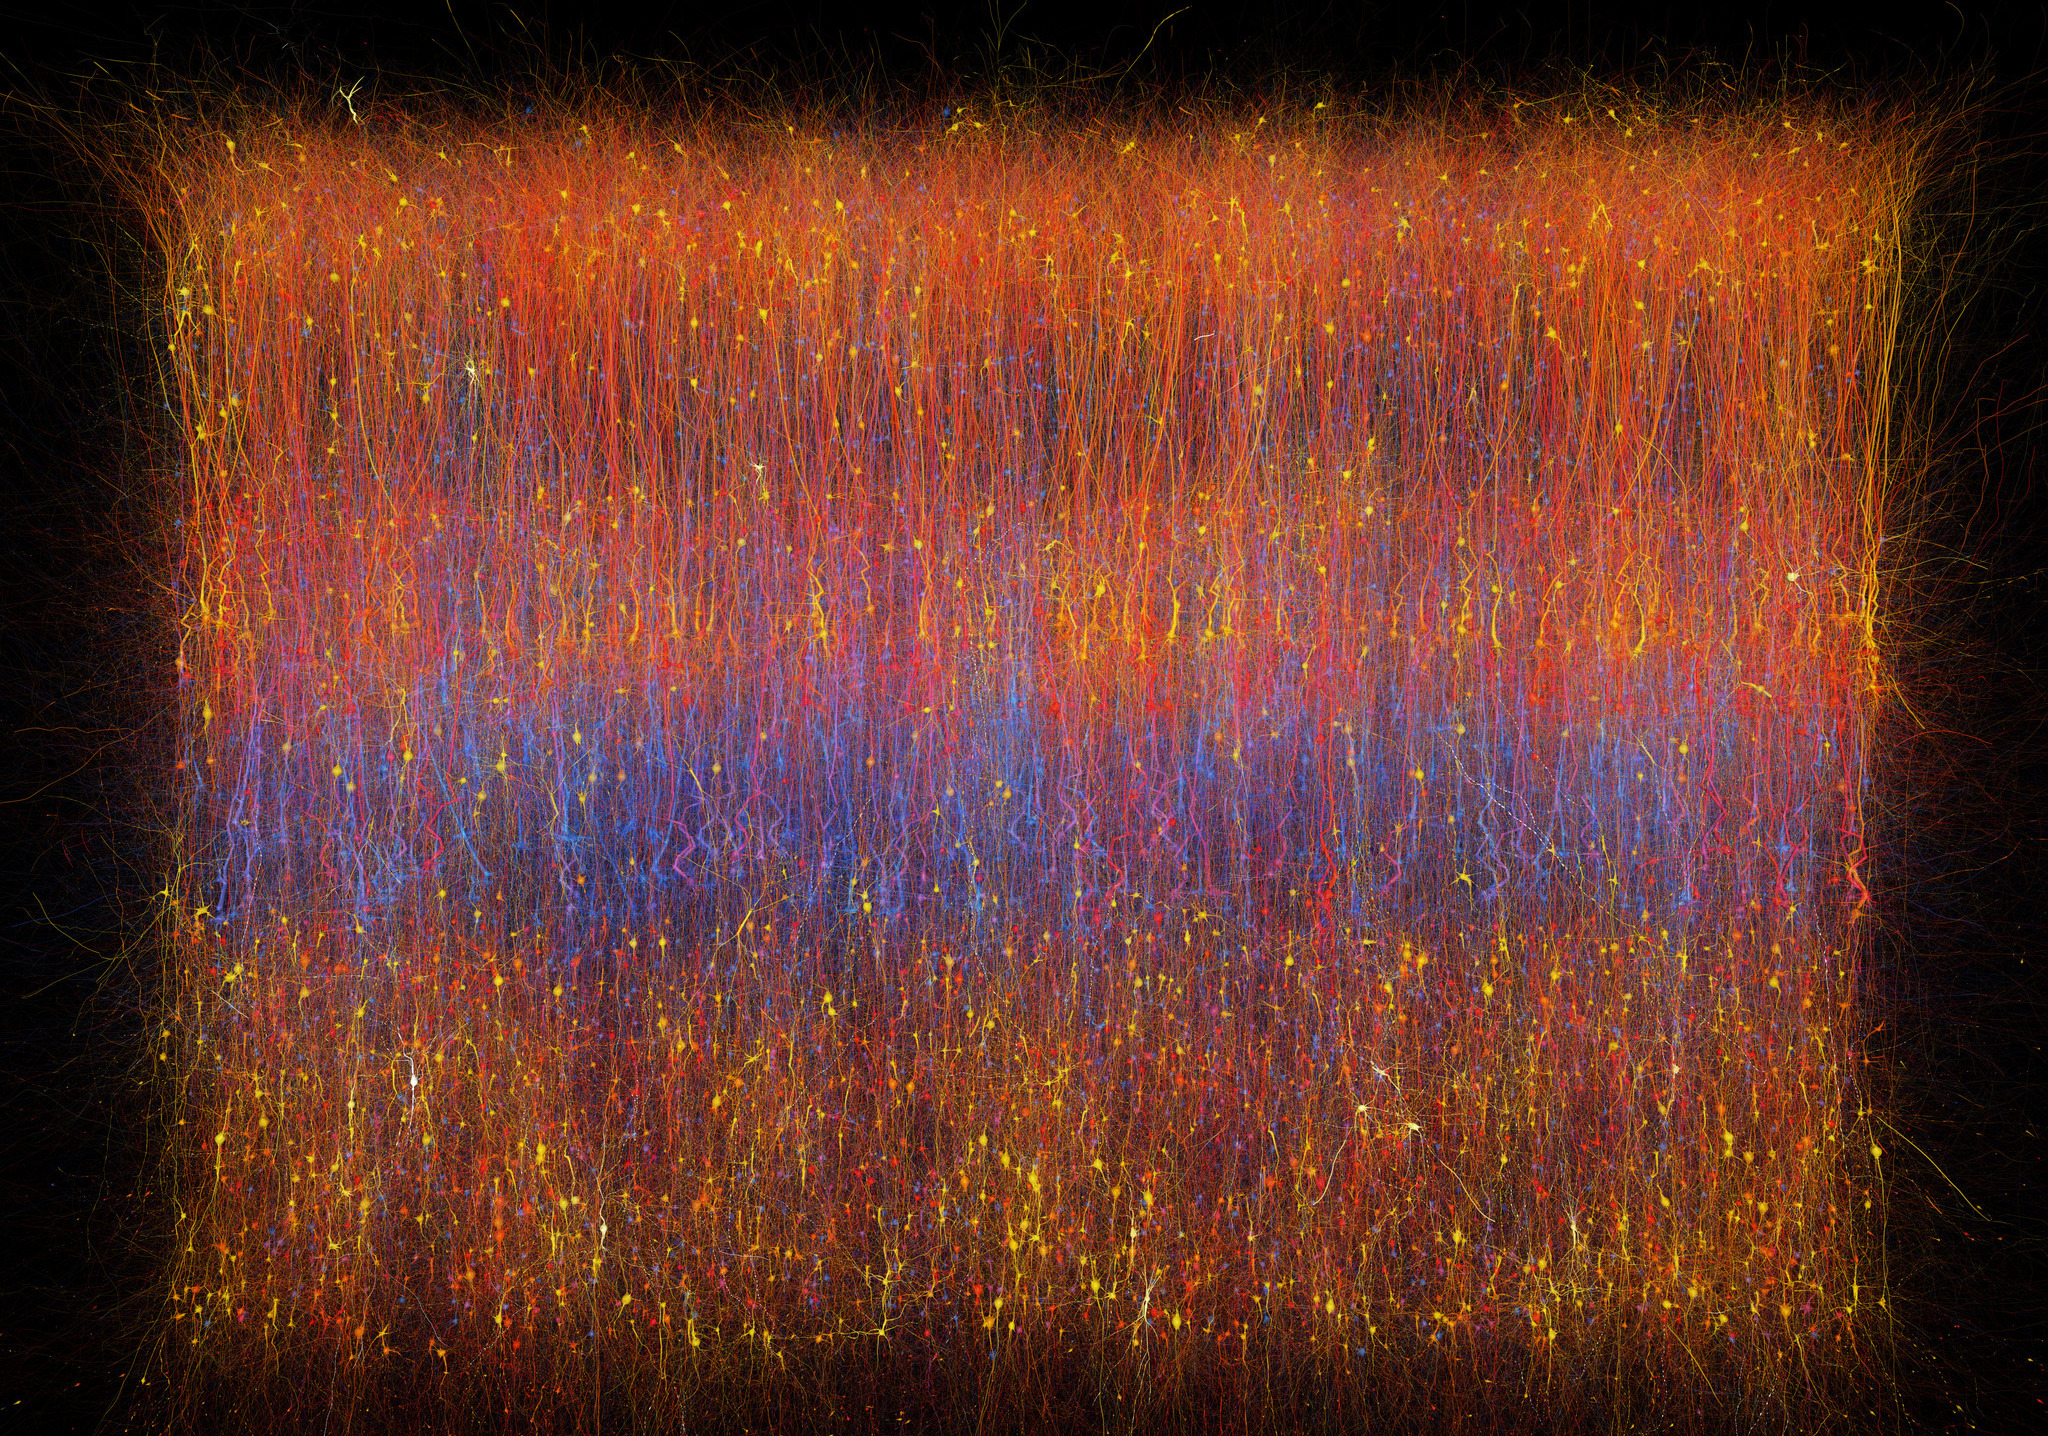
\includegraphics[height=5cm]{images/slices}\hfil%
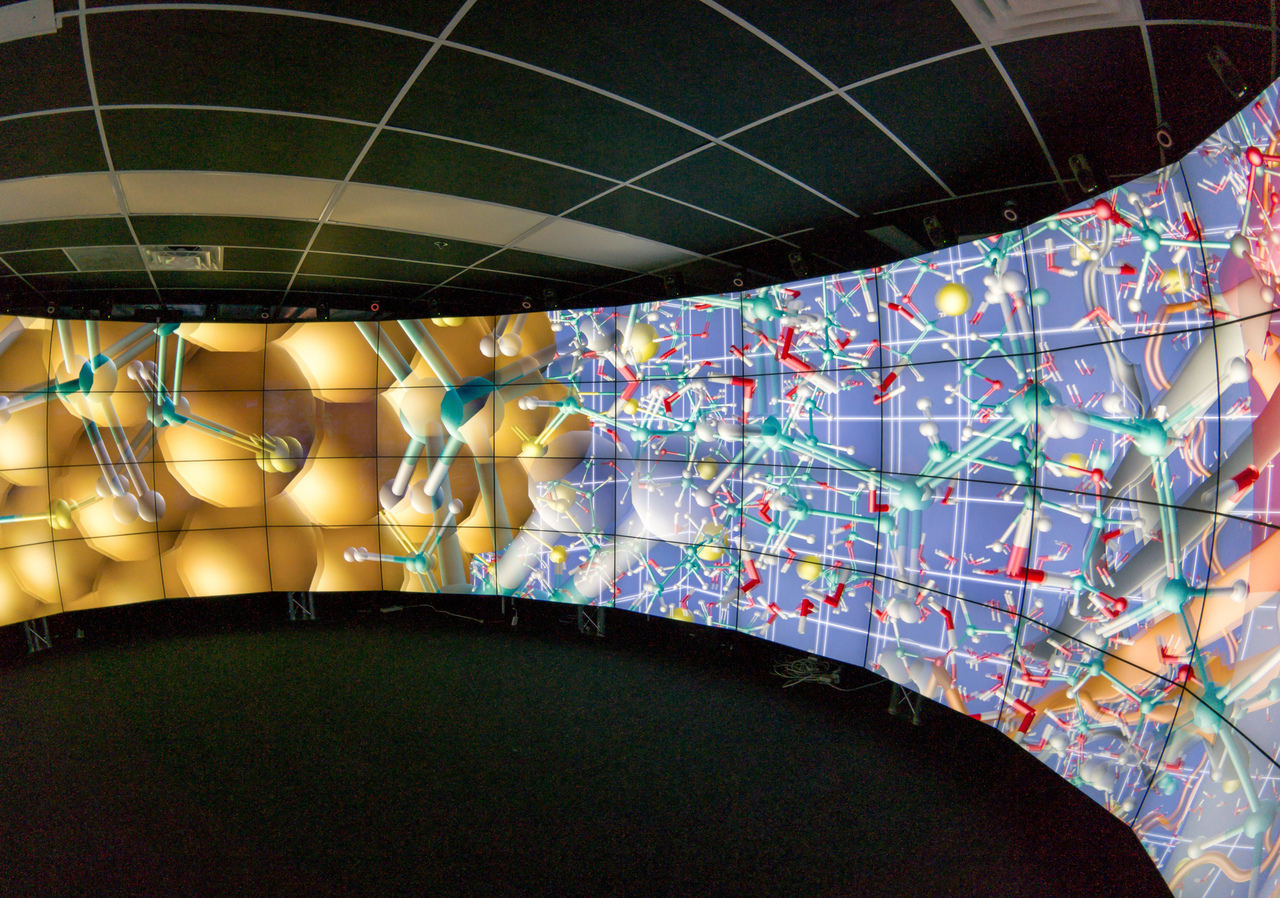
\includegraphics[height=5cm]{images/cave2}\\%
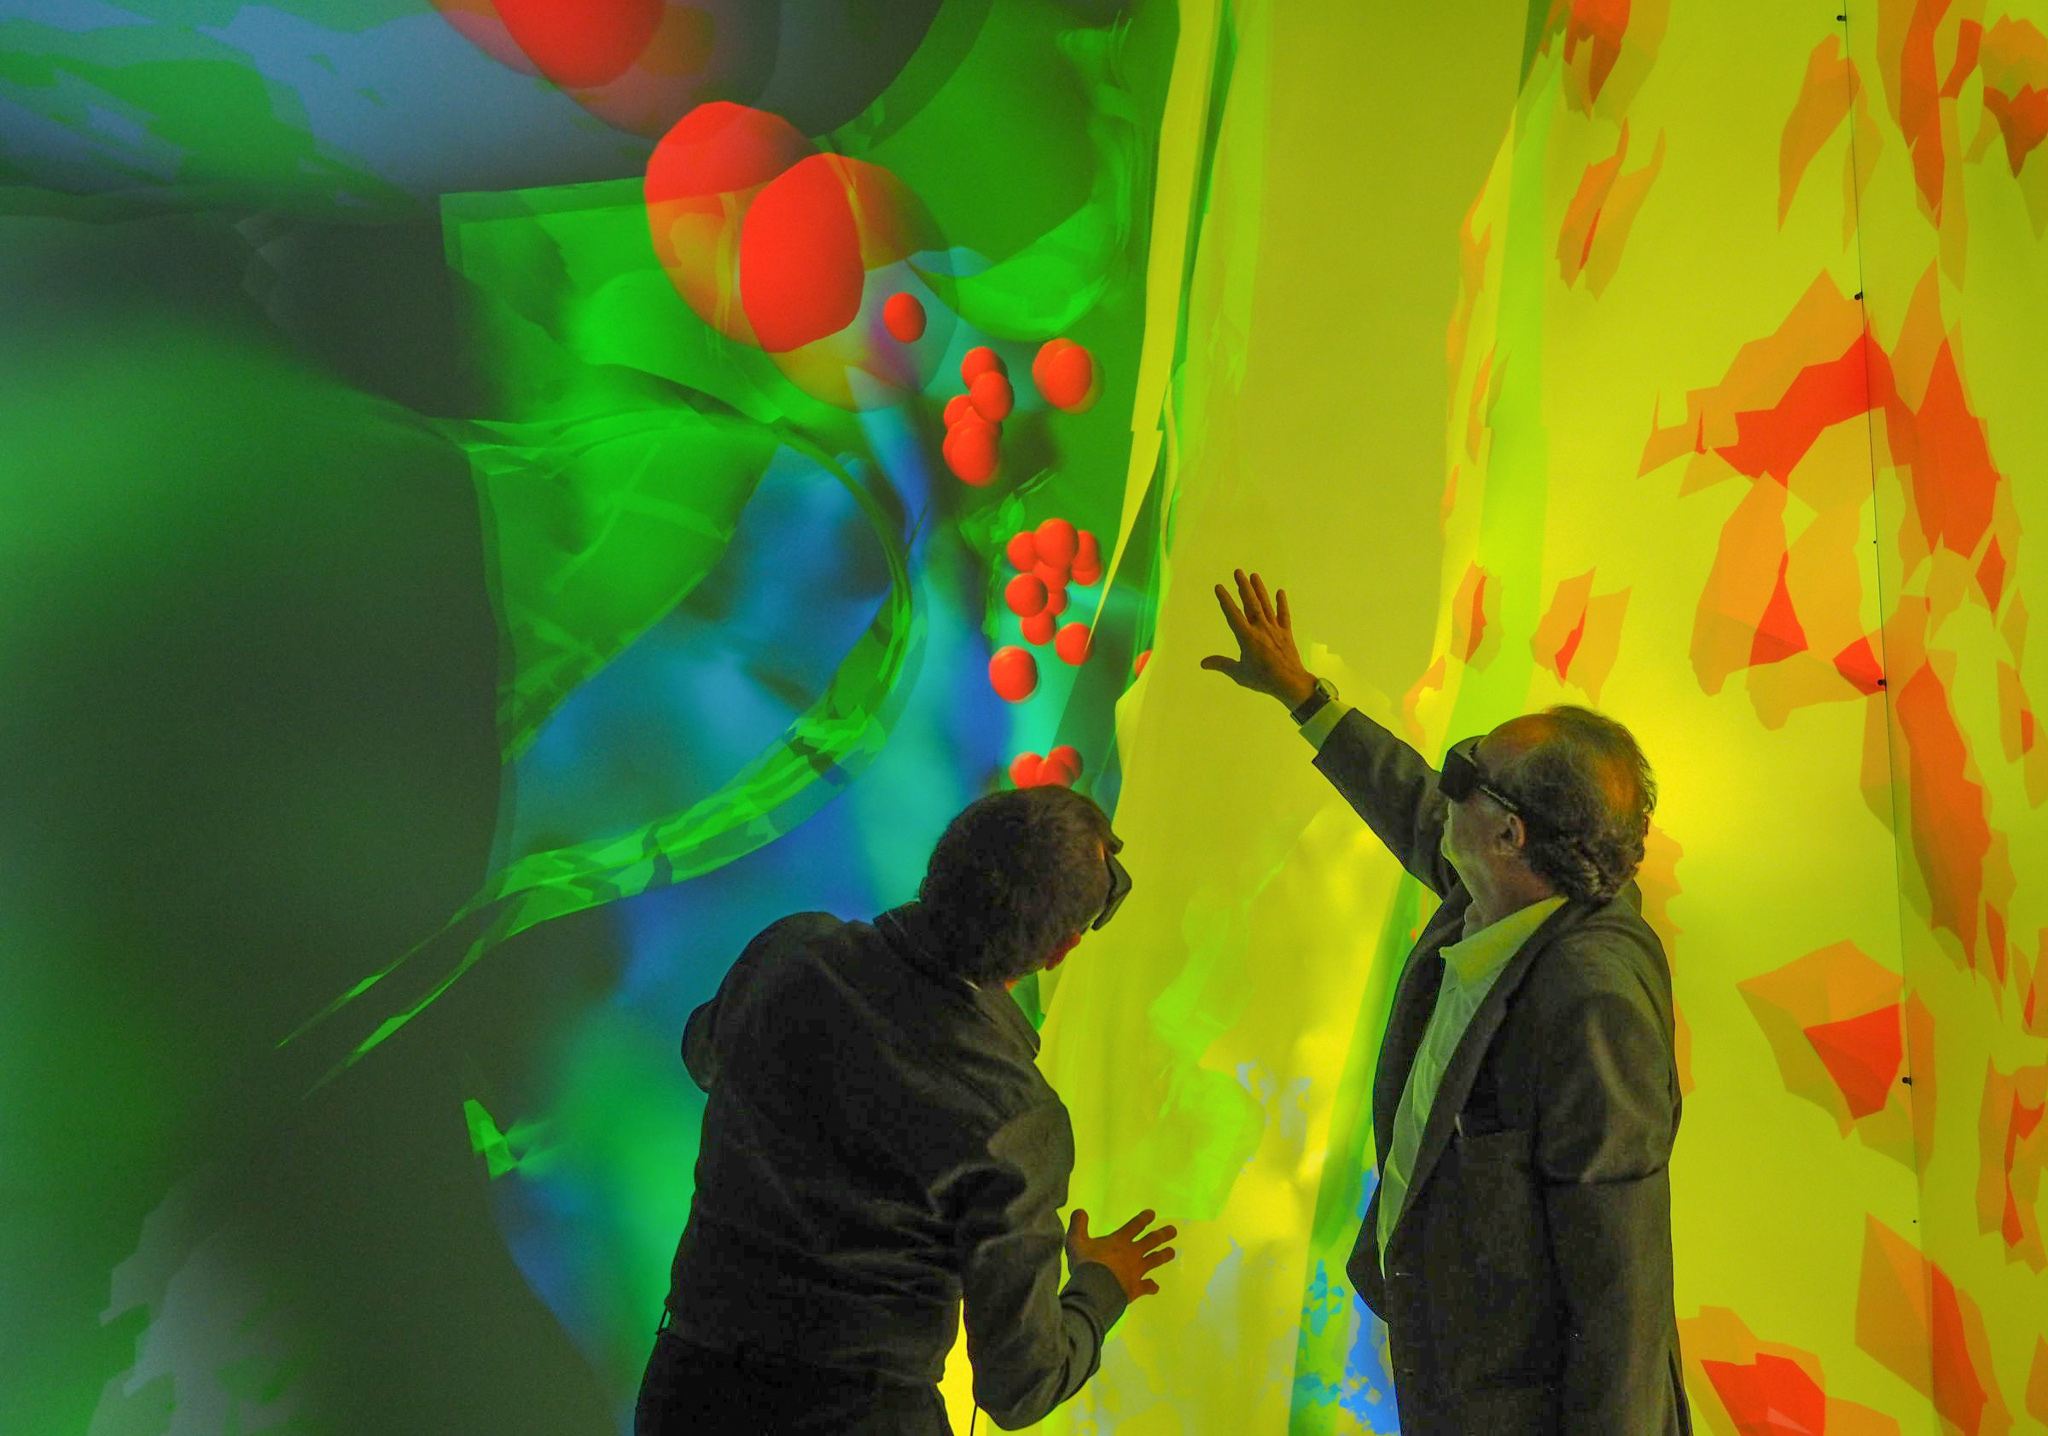
\includegraphics[height=5.27cm]{images/cave}\hfil%
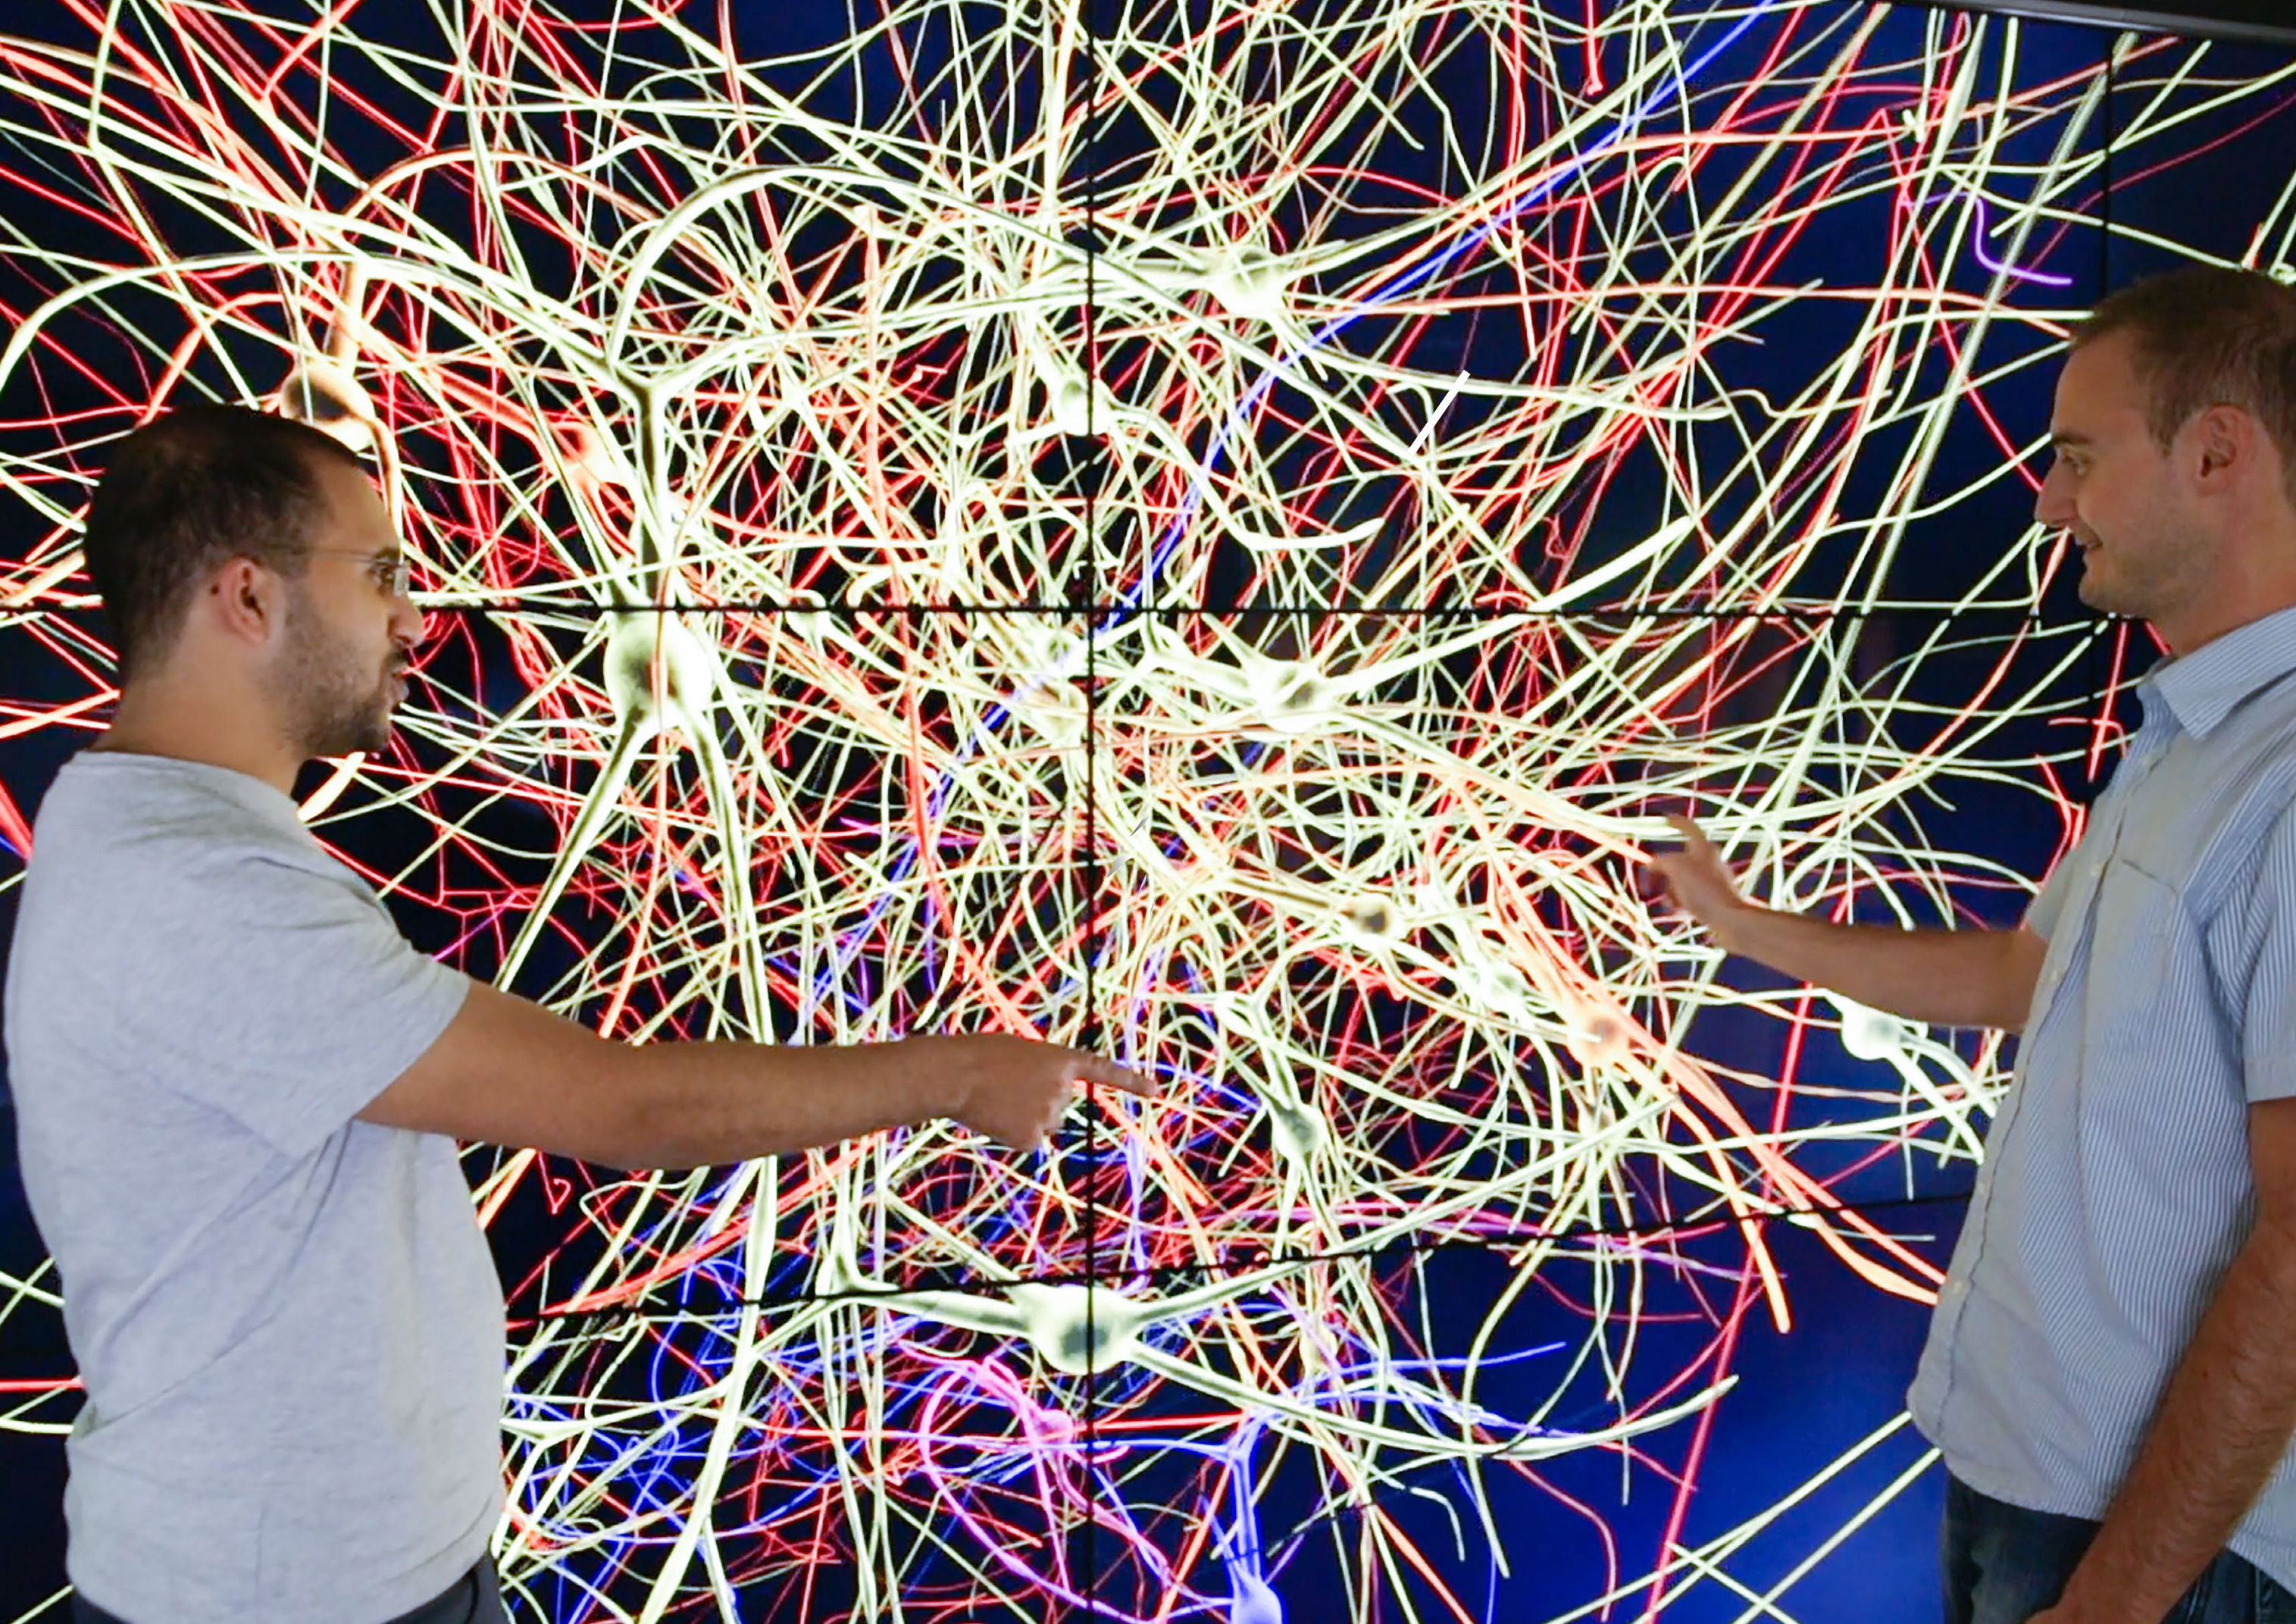
\includegraphics[height=5.27cm]{images/tide}%
\caption{Large Data Visualization: Large data visualization of a
      brain simulation, molecular visualization in the Cave$^2$, exploration of EM
      stack reconstructions in a Cave, collaborative data analysis on a tiled
      display wall.}
\end{figure}

Display technology has made significant progress in the last decade.
High-resolution screens and tiled display walls are now affordabe for most
organizations and are getting deployed at an increasing rate. This increased
resolution and display size helps with understanding the data, but with the
quadratic increase in pixels to be rendered, it increases the pressure on
rendering algorithms to deliver interactive framerates. Furthermore, for larger
system it becomes necessary to develop parallel and distributed applications.

However, not only applications are becoming more and more data-driven, but also
the technology used to tackle these kinds of problems is rapidly witnessing a
paradigm shift towards massively parallel on-chip and distributed parallel
cluster solutions. On one hand, parallelism within a system has increased
massively, with tenths of CPU cores, thousands of GPU cores and multiple CPUs
and GPUs in a single system. On the other hand, massively parallel distributed
systems are easily accessible from various cloud infrastructure providers, and
are also affordable for on-site hosting for many organizations.

System software to exploit the available hardware parallelism capable of
performing efficient interactive data exploration has not kept up with the pace
in hardware developments and data gathering capabilities. On one hand, this is
due to an inherent delay between hardware and software capabilities, since
development typically only starts once the hardware is available. On the other
hand, existing software engineered for different design parameters has a
significant inertia to change, to the extreme of the necessity to rewrite it
from scratch.

In the context of emerging data-intensive knowledge discovery and data analysis,
efficient interactive data exploration methodologies have become increasingly
important. Visual analysis by means of interactive visualization and inspection
of three-dimensional data is a particularly efficient approach to gain intuitive
insight into the spatial structure and relations of very large 3D data sets.
However, defining visual and interactive methods scalable with problem size and
degree of parallelism, as well as generic applicability of high-performance
interactive visualization methods and systems are recognized among the major
current and future challenges.

\section{Interactive Visualization}

\section{Parallel Rendering}

The main performance indicator for Large Data Interactive Rendering is the
performance of the rendering algorithm, that is, the framerate with which the
program produces new images. This framerate can be improved by either using
faster or more hardware, or by better algorithms exploiting the existing
hardware and data. This proposal primarily focuses on the first approach using
parallel rendering to exploit the CPU and GPU parallelism available on a single
system or a distributed cluster.  The early fundamental concepts have been laid
down in \cite{MCEF:94} and \cite{Crockett:97}. A number of domain specific
parallel rendering algorithms and special-purpose hardware solutions have been
proposed in the past, however, only few generic parallel rendering frameworks
have been developed (\fig{fSorts}). We will focus on sort-last and sort-first
rendering, since sort-middle architectures are only feasible in a hardware
implementation due to the large amount of fragments processed and transferred in
the sorting stage.

\begin{figure}[ht]\center
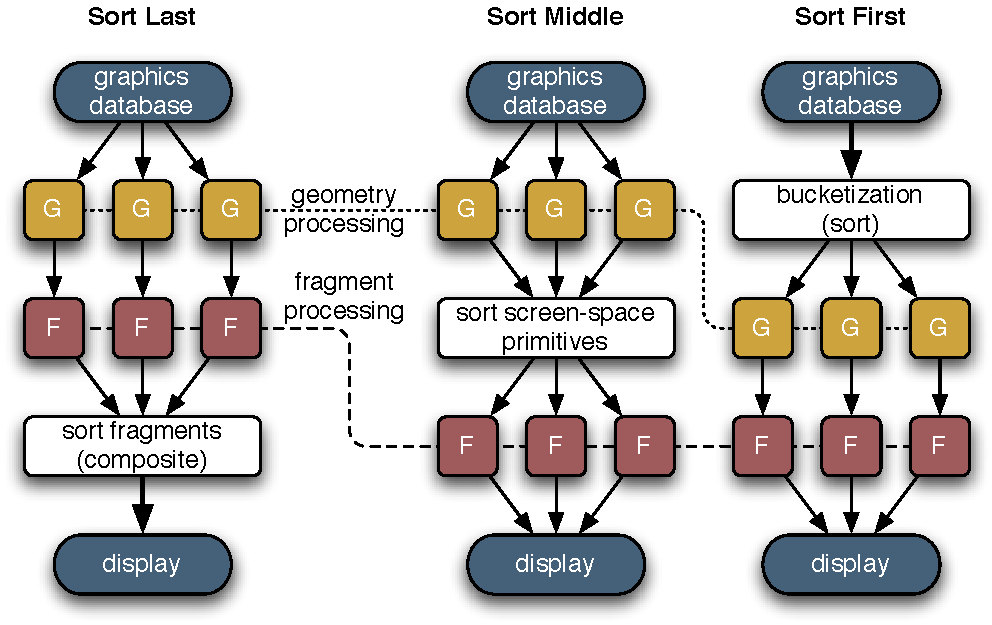
\includegraphics[width=0.7\textwidth]{images/all_sorts}%
\caption{Sort-last, sort-middle and sort-first parallel rendering\label{fSorts}}
\end{figure}


\subsection{Domain specific solutions}

Cluster-based parallel rendering has been commercialized for off-line rendering
(i.e. distributed ray-tracing) for computer generated animated movies or special
effects, since the ray-tracing technique is inherently amenable to
parallelization for off-line processing. Other special-purpose solutions exist
for parallel rendering in specific application domains such as volume rendering
\cite{LWMT:97,Wittenbrink:98,HSCSM:00,SL:02,GS:02,NSJLYZ:05} or
geo-visualization \cite{VR:91,AG:95,LDC:96,JLMV:06}. However, such specific
solutions are typically not applicable as a generic parallel rendering paradigm
and do not translate to arbitrary scientific visualization and distributed
graphics problems.

In \cite{NC:07}, parallel rendering of hierarchical level-of-detail (LOD) data
has been addressed and a solution specific to sort-first tile-based parallel
rendering has been presented. While the presented approach is not a generic
parallel rendering system, basic concepts presented in \cite{NC:07} such as load
management and adaptive LOD data traversal can be carried over to other
sort-first parallel rendering solutions.

\subsection{Special-purpose architectures}

Historically, high-performance real-time rendering systems have relied on an
integrated proprietary system architecture, such as the early SGI graphics super
computers. These special-purpose solutions have become a niche product as their
graphics performance does not keep up with off-the-shelf workstation graphics
hardware and scalability of clusters.

Due to its conceptual simplicity, a number of special-purpose image compositing
hardware solutions for sort-last parallel rendering have been developed. The
proposed hardware architectures include Sepia \cite {MHS:99a,sepia}, Sepia~2
\cite{LMSBHa:01,LMSBH:01}, Lightning~2 \cite{Stoll01}, Metabuffer
\cite{Blanke00,Zhang01}, MPC Compositor \cite{Muraki01} and PixelFlow
\cite{Molnar92, Eyles97}, of which only a few have reached the commercial
product stage (i.e. Sepia~2 and MPC Compositor). However, the inherent
inflexibility and setup overhead have limited their distribution and application
support. Moreover, with the recent advances in the speed of CPU-GPU interfaces,
such as PCI Express, NVLink and other modern interconnects, combinations of
software and GPU-based solutions offer more flexibility at comparable
performance.

\subsection{Generic approaches}

A number of algorithms and systems for parallel rendering have been developed in
the past. On one hand, some general concepts applicable to cluster parallel
rendering have been presented in \cite{Mueller:95,Mueller:97} (sort-first
architecture), \cite{SZFLS:99,SFLS:00} (load balancing), \cite{SFL:01} (data
replication), or \cite{CMF:05,CM:06} (scalability). On the other hand, specific
algorithms have been developed for cluster based rendering and compositing such
as \cite{AP:98}, \cite{CKS:02} and \cite{YYC:01,SMLAP:03}. However, these
approaches do not constitute APIs and libraries that can readily be integrated
into existing visualization applications, although the issue of the design of a
parallel graphics interface has been addressed in \cite{Igehy98}.

Only few generic APIs and (cluster-)parallel rendering systems exist which
include VR Juggler \cite{BJHMBC:01} (and its derivatives), Chromium
\cite{HHNFAKK:02} (an evolution of \cite{Humphreys99,Humphreys00,HEBSEH:01}),
{ClusterGL}~\cite{NHM:11} and OpenGL Multipipe SDK
\cite{JDBJBCER:04,BRE:05,MPK}. These approaches can be categorized into
transparent interception and distribution of the OpenGL command stream and into
the parallization of the application rendering code (\fig{fChromium}).

\begin{figure}[ht]
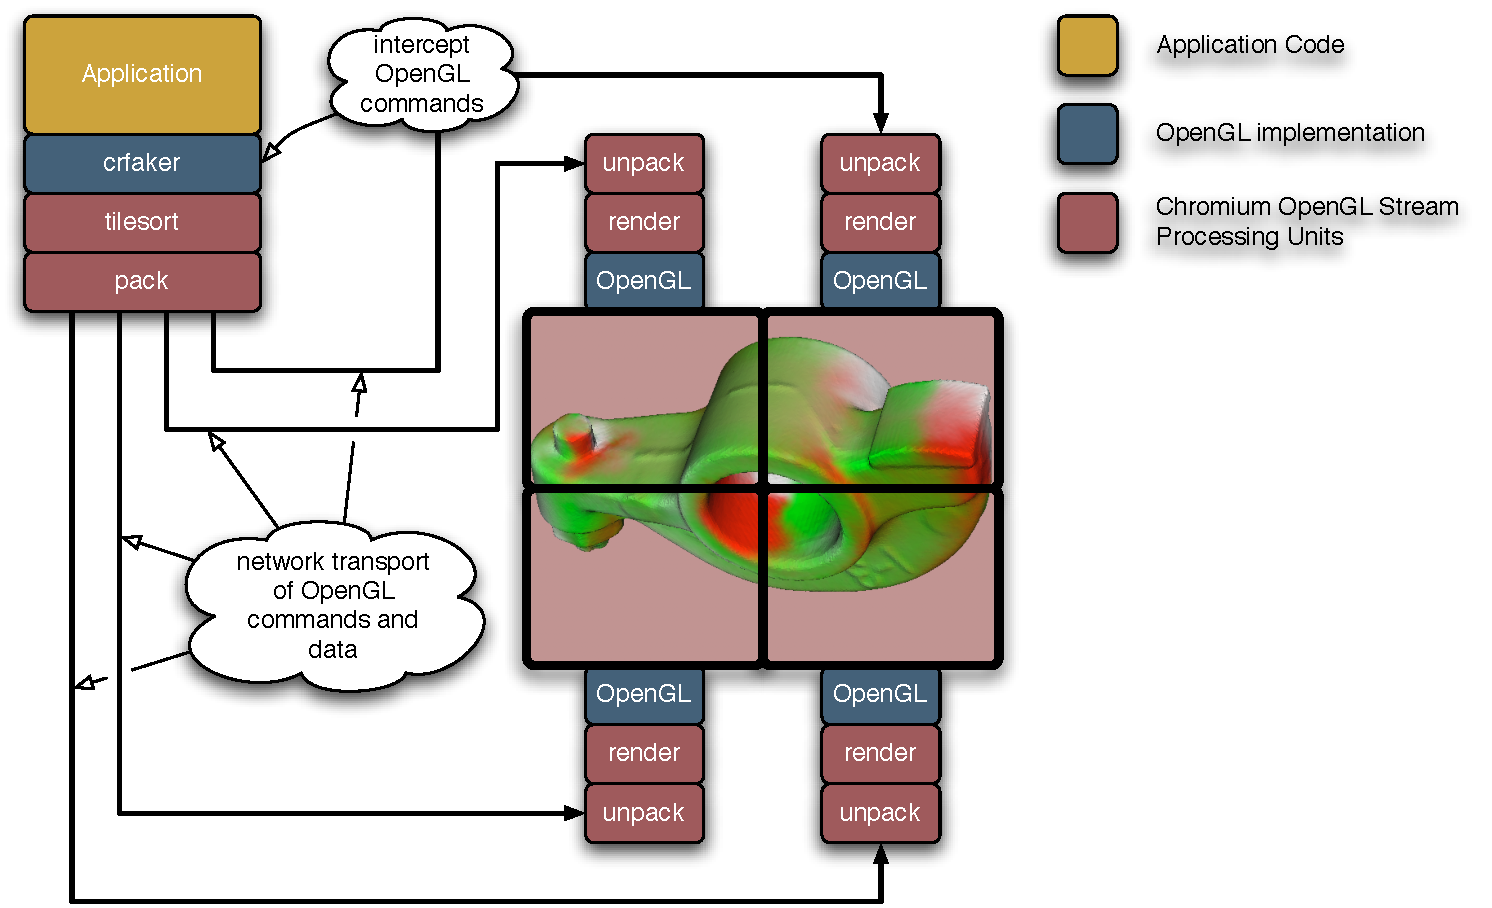
\includegraphics[height=4cm]{images/Chromium}\hfil%
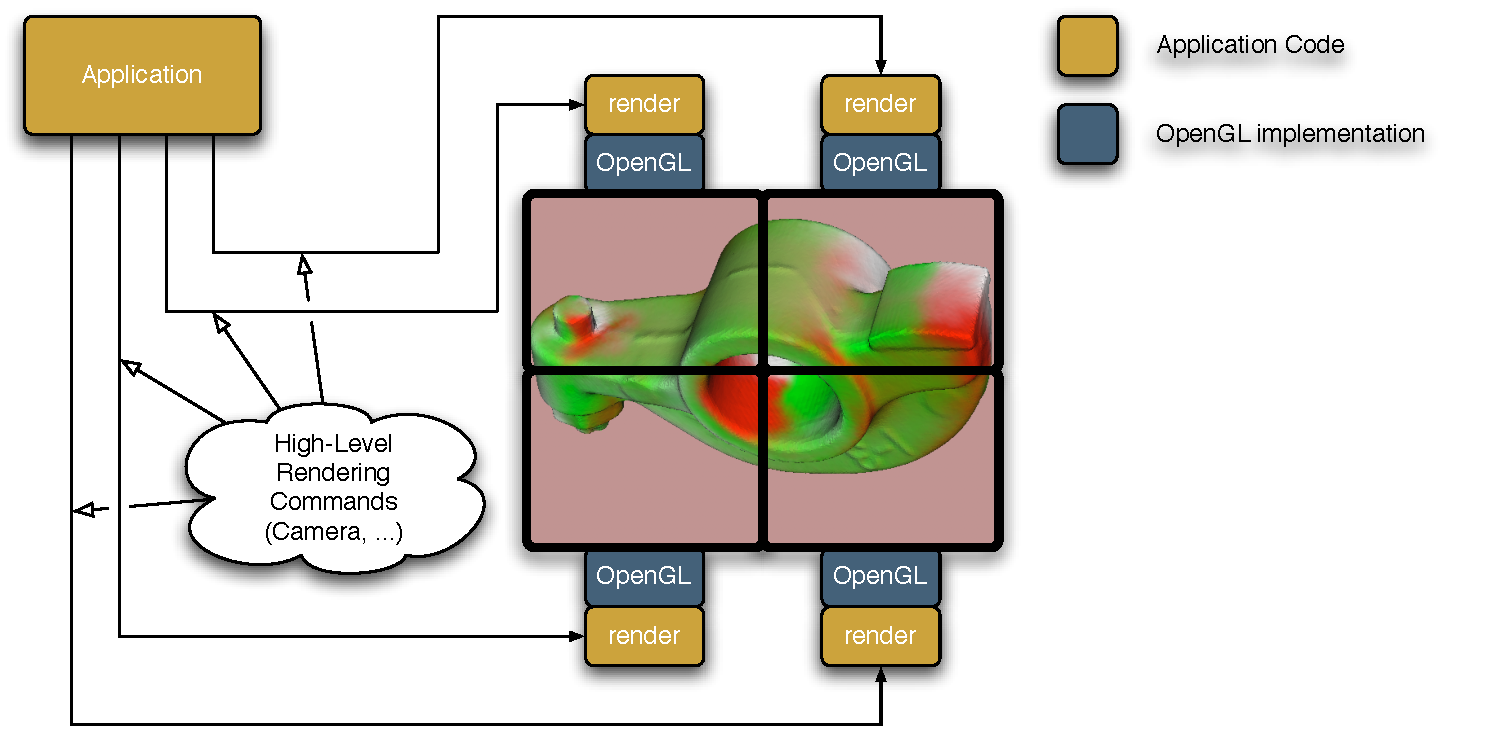
\includegraphics[height=4cm]{images/MPK}%
\caption{Transparent OpenGL interception and parallelization of the rendering code\label{fChromium}}
\end{figure}


VR Juggler \cite{BJHMBC:01,JBBC:98} is a graphics framework for virtual reality
applications which shields the application developer from the underlying
hardware architecture, devices and operating system. Its main aim is to make
virtual reality configurations easy to set up and use without the need to know
details about the devices and hardware configuration, but not specifically to
provide scalable parallel rendering. Extensions of VR Juggler, such as for
example ClusterJuggler \cite{BC:03} and NetJuggler \cite{AGLMR:02}, are
typically based on the replication of application and data on each cluster node
and basically take care of synchronization issues, but fail to provide a
flexible and powerful configuration mechanism that efficiently supports scalable
rendering as also noted in \cite{SWNH:03}. VR Juggler does not support scalable
parallel rendering such as sort-first and sort-last task decomposition and image
compositing nor does it provide support for network swap barriers
(synchronization), distributed objects, image compression and transmission, or
multiple rendering threads per process, important for multi-GPU systems.

While Chromium \cite{HHNFAKK:02} provides a powerful and transparent abstraction
of the OpenGL API, that allows a flexible configuration of display resources,
its main limitation with respect to scalable rendering is that it is focused on
streaming OpenGL commands through a network of nodes, often initiated from a
single source. This has also been observed in \cite{SWNH:03}. The problem comes
in when the OpenGL stream is large in size, due to not only containing OpenGL
calls but also the rendered data such as geometry and image data. Only if the
geometry and textures are mostly static and can be kept in GPU memory on the
graphics card, no significant bottleneck can be expected as then the OpenGL
stream is composed of a relatively small number of rendering instructions.
However, as it is typical in real-world visualization applications, display and
object settings are interactively manipulated, data and parameters may change
dynamically, and large data sets do not fit statically in GPU memory but are
often dynamically loaded from out-of-core and/or multiresolution data
structures. This can lead to frequent updates not only of commands and
parameters wich have to be distributed but also of the rendered data itself
(geometry and texture), thus causing the OpenGL stream to expand dramatically.
Furthermore, this stream of function calls and data must be packaged and
broadcast in real-time over the network to multiple nodes for each rendered
frame. This makes CPU performance and network bandwidth a more likely limiting
factor.

The performance experiments in \cite{HHNFAKK:02} indicate that Chromium is
working quite well when the rendering problem is fill-rate limited. This is due
to the fact that the OpenGL commands and a non-critical amount of rendering data
can be distributed to multiple nodes without significant problems and since the
critical fill-rate work is then performed locally on the graphics hardware.

Chromium also provides some facilities for parallel application development,
namely a sort-last, binary-swap compositing SPU and an OpenGL extension
providing synchronization primitives, such as a barrier and semaphore. It leaves
other problems, such as configuration, task decomposition as well as process and
thread management unaddressed. Parallel Chromium applications tend to be written
for one specific parallel rendering use case, such as for example the sort-first
distributed memory volume renderer \cite{BHPB:03} or the sort-last parallel
volume renderer raptor \cite{Raptor}. We are not aware of a generic
Chromium-based application using many-to-one sort-first or stereo
decompositions.

The concept of transparent OpenGL interception popularized by WireGL and
Chromium has received some further contributions. While some commercial
implementations such as {TechViz} and {MechDyne Conduit} continue to exist, on
the research side only {ClusterGL}~\cite{NHM:11} has been presented recently.
{ClusterGL} employs the same approach as {Chromium}, but delivers a
significantly faster implementation of transparent OpenGL interception and
distribution for parallel rendering. Transparent OpenGL interception is an
appealing apporach for some applications since it requires no code changes, but
it has inherent limitiations due to the fact that eventually the bottleneck
becomes the single-threaded application rendering code, the amount of
application data the single application instance can load or process, or the the
size of the OpenGL command stream send over the network.

{CGLX}~\cite{DK:11} tries to bring parallel execution transparently to
OpenGL applications, by emulating the GLUT API and intercepting certain OpenGL
calls. In contrast to frameworks like {Chromium} and {ClusterGL}
which distribute OpenGL calls, {CGLX} follows the distributed application
approach. This works transparently for trivial applications, but quickly
requires the application developer to address the complexities of a distributed
application, when mutable application state needs to be synchronized across
processes. For realistic applications, writing parallel applications remains the
only viable approach for scalable parallel rendering, as shown by the success of
{Paraview}, {Visit} and {Equalizer}-based applications.

OpenGL Multipipe SDK (MPK) \cite{BRE:05} implemented an effective parallel
rendering API for a shared memory multi-CPU/GPU system. It is similar to IRIS
Performer \cite{RH:94} in that it handles multi-GPU rendering by a lean
abstraction layer via a conceptual callback mechanism, and that it runs
different application tasks in parallel. However, MPK is not designed nor meant
for rendering nodes separated by a network. MPK focuses on providing a parallel
rendering framework for a single application, parts of which are run in parallel
on multiple rendering channels, such as the culling, rendering and final image
compositing processes.

Software for driving and interacting with tiled display walls has received
significant attention, including {Sage}~\cite{Sage} and
{Sage~2}~\cite{Sage2} in particular. {Sage} was built entirely
around the concept of a shared framebuffer where all content windows are
separate applications using pixel streaming but is no longer actively supported.
{Sage 2} is a complete, browser-centric reimplementation where each
application is a web application distributed across browser instances.
{DisplayCluster}~\cite{DisplayCluster}, and its continuation
{Tide}~\cite{tide}, also implement the shared framebuffer concept of
{Sage}, but provide a few native content applications integrated into the
display servers. These solutions implement a scalable display environment and
are a target display platform for scalable 3D graphics applications.

\section{Dissertation Structure}


\chapter{Contributions}

\section{Generic Parallel Rendering Framework}

\section{Parallel Rendering Modes}

\section{Load Balancing}

\section{Applications}


\chapter{Parallel Rendering Framework Architecture}

\section{Overview}
A generic parallel rendering framework has to cover a wide range of use cases,
target systems, and configurations. This requires on one hand a strong
separation between the implementation of an application and its configuration,
and on the other hand a careful design to allow the resulting program to scale
up to hundreds of nodes, while providing a minimally invasive API for the
developer. In this section we present the system architecture of the Equalizer
parallel rendering framework, and motivate its design in contrast to related
work.

The motivation to use parallel rendering is either driven by the need to drive
multiple displays or projectors from multiple GPUs and potentially multiple
nodes, or by the need to increase rendering performance to be able to visualize
more data or use a more demanding rendering algorithm for higher visual quality.
Occasionally both needs coincide, for example for the analysis for large data
sets on high fidelity visualization systems.

Fundamentally, there are two approaches to enable applications to use multiple
GPUs: transparent interception at the graphics API (typically OpenGL) or
extending the application to support parallel rendering natively. The first
approach has been extensively explored by Chromium and others, while the second
is the foundation for this thesis. The architecture of Equalizer is founded on
an in-depth requirements analysis of typical visualization applications,
existing frameworks, and previous work on OpenGL Multipipe SDK.

The task of parallelizing a visualization application boils down to configuring
the application's rendering code differently for each resource, enabling this
rendering code to access the correct data, and synchronizing execution. For
scalable rendering, when multiple GPUs are used to accelerate a single output,
partial results need to be collected from all contributing resources and
combined on the output. Equalizer has a strong seperation of the rendering code
from its runtime configuration. The configuration is layed out in a hierarchical
resource description and compound trees configuring the resources for parallel
and scalable rendering. The configuration is a dynamic runtime structure, with a
serialized configuration file format.

In the following we will first describe the execution model and runtime
configurability, followed by the how the generic configuration is used to model
the desired visualization setup, and finally introduce specifics of scalable and
distributed rendering.

\section{Asynchronous Execution Model}

The core execution model was pioneered by CAVELib \cite{DACNCCGHPSNS:97},
refined by OpenGL Multipipe SDK for shared memory systems, and substantially
extended by Equalizer for asynchronous and distributed execution. By analysing
the typical architecture of a visualization application we observer an
initialization phase, a main rendering loop, and an exit phase. Equalizer
decomposes these steps for parallel executions.

The main rendering loop typically consists of four phases: submitting the
rendering commands to the graphics subsystem, displaying the renderered image,
and retrieving events from the operating system, based on which the application
state is updated and a new image is rendered. The configuration of the rendering
is largely hard-coded, with a few configurables such as field of view or stereo
separation. For parallel execution, we need to separate the rendering code from
this main loop, and execute it in parallel with different rendering parameters,
as shown in \fig{FIG_execution}. Similarly, the initialization and exit phase
also needs to be decomposed to allow managing multiple, distributed resources.

\begin{figure}[ht]\center
  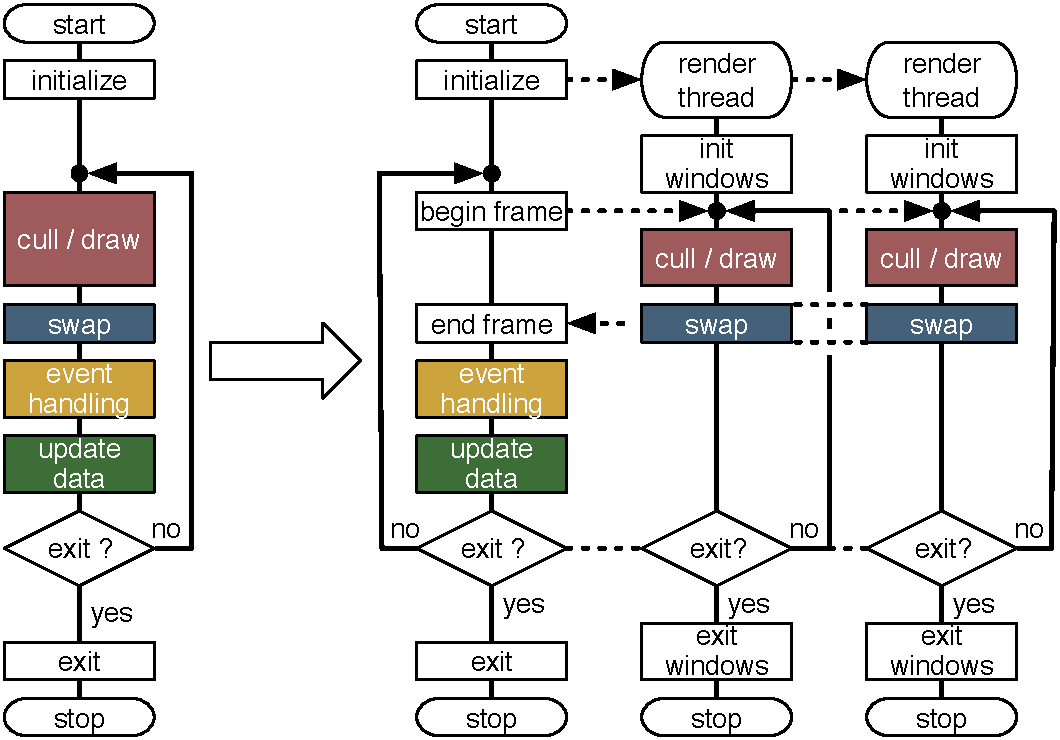
\includegraphics[width=.9\columnwidth]{images/executionFlow}
  \caption{Simplified execution flow of a classical visualization application
    and an Equalizer application.}
  \label{FIG_execution}
\end{figure}

Without going into the details at this point, another critical design parameter
are synchronization points. Most implementations use a per-frame barrier or
similar synchronization to manages parallel execution. In larger installations,
this is detrimental for scalability, as even slight load imbalances limit
parallel speedup. The Equalizer execution model is fully asynchronuous, and only
introduces synchronization points when strictly needed. The main synchronization
points are: configured swap barriers between a set of output which have to
display simultaneously, the availability of input frames for scalable rendering,
and a task synchronization to prevent runaway of the main loop execution. By
default, Equalizer keeps up to one frame of latency in execution, that is, some
resource might render the next frame while others are still finishing the
current. Nonetheless, resources which are ready will immediately display their
result. The asynchronous execution architecture, coupled with a frame of
latency, allows pipelining of many operations, such as the application event
processing, task computation and load balancing, rendering, image readback,
compression, network transmission, and compositing.


\subsection{Programming Interface}

Equalizer provides a framework to facilitate the development of distributed as
well as non-distributed parallel rendering applications. The programming
interface is based on a set of C++ classes, modeled closely to the resource
hierarchy of a graphics rendering system. The application subclasses these
objects and overrides C++ task methods, similar to C callbacks. These task
methods will be called in parallel by the framework, depending on the current
configuration. This parallel rendering interface is significantly different from
Chromium \cite{HHNFAKK:02} and more similar to VRJuggler \cite{BJHMBC:01} or
OpenGL Multipipe SDK \cite{BRE:05}.

\subsection{Application}

The main application thread in Equalizer drives the rendering, that is, it
carries out the main rendering loop, but does not actually execute any
rendering. Depending on the configuration, the application process often hosts
one or more render client threads. When a configuration has no additional nodes
besides the application node, all application code is executed in the same
process, and no network data distribution has to be implemented. The main
rendering loop is quite simple: The application requests a new frame to be
rendered, synchronizes on the completion of a frame and processes events
received from the render clients. Figure~\ref{FIG_execution} shows a simplified
execution model of an Equalizer application.


\subsection{Server}

The Equalizer server manages the parallel rendering session. It is an
asynchronous execution thread or process which receives requests from the
application and serves these requests using the current configuration, launching
and stopping rendering client processes on nodes, determining the rendering
tasks for a frame, and synchronizing the completion of frames.

\subsection{Render Client}

During initialization of the server, the application provides a rendering
client. The rendering client is often, especially for simple applications, the
same executable as the application. However, in more sophisticated
implementations the rendering client can be a smaller executable which only contains
the application-specific rendering code. The server deploys this rendering
client on all nodes specified in the configuration.

In contrast to the application process, the rendering client does not need to
have a main loop and is completely controlled by the Equalizer framework based
on application commands. If a configuration also uses the application node for
rendering then the rendering happens in different threads within the application
process. A render client consists of the following threads: the node main
thread, one network receive thread, and one thread for each graphics card (GPU)
to execute rendering tasks.

The Equalizer client library implements the main loop, which receives network
events, processes them, and invokes the necessary task methods provided by the
developer.

Most importantly, the network data contains the rendering task
parameters computed by the server. Based on this data, the client library sets
up the rendering context and calls the application-provided task methods.
Setting up the rendering context consists of using the correct rendering thread,
making the drawable and graphics context current, as well as providing the task
methods with the 2D viewport, frustum, view matrix and the data-range for
sort-last rendering. The task methods clear the frame buffer as necessary,
execute the OpenGL rendering commands as well as readback, and assemble partial
frame results for scalable rendering. All tasks have default implementations so
that only the application specific methods have to be implemented, which
typically includes the {\tt frameDraw()} method. For example, the default
callbacks for frame recomposition during scalable rendering implement tile-based
assembly for sort-first and stereo decompositions, and $z$-buffer or compositing
for sort-last rendering of polygonal data.
% or back-to-front $\alpha$-blending for direct volume rendering.
% eile: back-to-front is not implemented in Eq, since the order is
% app-specific. It can be implement easily though, as demonstrated with eVolve.
A detailed description of the API and all methods can be found in the programming
guide \cite{Eilemann:07}.

Event handling is implemented by listening asynchronously for events
from all windows. Events are transformed from window-system specific
events into generic window events, and dispatched to the correct
window. The window either processes the event locally, or converts it
into a config-event to be sent to the application node. The application
node processes the config-events as part of its main rendering loop. A
more detailed description of event handling can also be found in \cite {Eilemann:07}.

In addition to executing the application code in the right context, the
client library implements image compression and transmission, network
swap barrier support and distributed object support.

\subsubsection{Render Context}

\section{Configuration}
\subsection{Rendering Resources}
\subsection{Display Resources}
\subsection{Compounds}

\section{Compositing}

\section{Load Balancing}

\section{Distribution Layer}


\chapter{New Parallel Rendering Modes}


\chapter{Compositing Optimisations}


\chapter{New Load Balancing Algorithms}


\chapter{Data Distribution and Synchronization}


\chapter{Conclusion}

\section{Future Work}


\if 0

\chapter{Problem Statement}

Visualization of large amounts of data has been always been encumbered by
sufficient system software. Compared to other domains, such as HPC simulations,
large data visualization has received relatively little attention in both
research and development. Consequently, there is a large amount of data which
has not been explored sufficiently. In particular in scientific visualization,
where data is often spatial and temporal, even simple visualizations can extract
new information and provide a valuable tool to domain scientists for discovery.

The central theme of the proposed research is therefore: {\bf How can we improve
the capabilities of existing visualization algorithms for rendering large
amounts of data?} This generic problem can be researched more concretely along
the following research questions:
\begin{compactenum}
\item How can we improve the rendering performance of visualization applications to enable users to explore more data?
    \begin{compactenum}
    \item What new algorithms will decrease the time needed to composite rendering results, in particular for sort-last rendering?
    \item How can we improve load-balancing for sort-first rendering, in particular for large display systems?
    \end{compactenum}
\item How can we reduce end-to-end system latency for better user experience?
    \begin{compactenum}
    \item In a generic parallel rendering framework, how can we schedule the different rendering stages to minimize the latency for the user?
    \item How can we architect the parallel rendering framework to minimize synchronization between threads?
    \end{compactenum}
\item How can we maximize the impact of this research on large data scientists?
\end{compactenum}

The obvious solution to the problem is to utilize more compute resources to
parallelize and scale the rendering algorithm. The goal can either be to
increase strong scaling (render a given data set faster) or weak scaling (render
a larger data set at roughly the same speed). To efficiently use more resources,
we need to research increasing the parallelism of existing algorithms, and to
reduce the bottleneck in the image compositing stage.

An important collateral problem is the overall latency of the rendering system,
that is, the time between a user input and its resulting output frame. While
this is lower-bounded by the framerate of the rendering, oftentimes algorithmic
or implementation choices increase the total system latency. Often this is a
side effect of improving the rendering performance, but it also decreases the
usability of the application for interactive usage. One typical example is
pipelining of operations in the rendering pipeline.

Visualizing large amounts of data often goes hand in hand with the usage of
high-resolution displays. Since large amounts of data tends to have a lot of
detail, high-resolution desktop screens (4K or 8K resolution), as well as
high-resolution display walls, help tremenduously in recognising and
understanding details of the data. The high resolution however aggravetes all
the aforementioned problems: The increased pixel count reduces rendering
performance, requires better compositing algorithms, and increases the latency
due to longer transfer times during compositing and display. Since pixel count
increases quadratically with display size, this problem will become more
important as display resolution increases.

\chapter{Proposed Solution} % 2-6

Parallel rendering has received a lot of attention in the last couple of
decades, yet libraries and frameworks to develop parallel rendering applications
are scarcely available. Consequently, there are only a few applications which
can utilize parallelism for rendering, let alone do so efficiently at scale.
This research proposes to address these shortcomings by developing {\bf reusable
software components} to make parallel rendering programs easier to develop, by
generalizing existing research into reusable software implementations.

Based on these foundations, we propose to research new algorithms to improve
rendering performance. In particular we see potential in improving the
scalability through better {\bf load balancing}, {\bf image compositing}
algorithms, and {\bf holistic optimization} of the whole rendering pipeline
under control of our framework. Orthogonally to this algorithmic research, we
propose to research {\bf data processing and data access} strategies for
parallel rendering applications. This is particularly important, yet
underdeveloped, in the context of the visual analysis for HPC simulation
results.

Previous parallel rendering approaches typically failed in one of the following
system requirements:
%
\begin{compactenum}
\item generic application support, instead of domain-specific solution
\item scalable abstraction of the graphics layer
\item exploit existing code infrastructure, such as proprietary scene graphs, molecular data structures, level-of-detail and geometry databases
\end{compactenum}

To date, generic and scalable parallel rendering frameworks that can be adopted
to a wide range of scientific visualization domains are not yet readily
available. Furthermore, flexible configurability to arbitrary cluster and
multi-display configurations has also not been addressed in the past, but is of
immense practical importance to scientists depending on high-performance
interactive visualization as a scientific tool. We propose a novel flexible
framework for parallel rendering that supports scalable performance,
configuration flexibility, is minimally invasive with respect to adapting
existing visualization applications, and is applicable to virtually any
scientific visualization application domain.

To that end, this work aims to significantly advance the system design and
implementation of flexible, distributed and cluster-parallel rendering
frameworks as well as algorithms and system design for large data processing in
the context of interactive visualization. The core of this proposal is the
Equalizer project, a foundation for scalable, multi-GPU visualization software
in all application domains. The main contributions of such a parallel rendering
system are:
%
\begin{compactenum}
\item novel concept for flexible runtime configuration of graphics system resources
\item easy specification of parallel task decomposition and image compositing algorithms
\item automatic decomposition and distributed execution of rendering tasks according to the configuration
\item support for polygonal and volume rendering for opaque and transparent geometries
\item fully decentralized software architecture providing network swap barrier synchronization and data distribution functionality
\item support for low-latency distributed frame synchronization and image compositing
\item minimally invasive programming model
\end{compactenum}

The broader impact of this work revolves around the development and improvement
of a generic, flexible and scalable parallel rendering infrastructure applicable
to a large number of application domains. The expected improvements of the
proposed activities in distributed parallel parallel rendering will be
integrated into open source software libraries and as such will be available to
the general public and especially to developers of high-performance
visualization and interactive rendering applications. This approach will
maximize the impact of this research on large data scientists (research question
4).

A strong focus during the development is to architect the framework for
scalability to address research questions 1 and 2. Based on my previous work and
the study of existing implementations, scalability in parallel rendering today
is mostly limited by excessive synchronization between execution threads,
imbalance in the task decomposition, and compositing performance. Equalizer only
has the following necessary synchronization points:
%
\begin{compactenum}
\item Swap synchronization between output channels to the same display system
\item Finalization of rendering frames given a configurable latency for all render threads
\item Availability of image data for compositing between the source and destination threads
\end{compactenum}
%
This architecture has proven to provide good scalability by inherently allowing
the pipelining of data synchronization, rendering and compositing tasks
(research question 1), while simultaneously minimizing the time to display
results by letting render threads execute as early as possible (research
question 2). Furthermore, this will provide better scalability for the more
specific research questions 1(a) and 1(b).

The following publications are planned or already published to address the corresponding research question:
\begin{compactenum}
    \item
    \begin{compactenum}
        \item In \cite{EP:07, MEP:10, EBAHMP:12} we presented different algorithms to optimize the compositing step for sort-last rendering and optimisations for modern multi-GPU NUMA nodes.
        \item In \cite{EEP:11, SPEP:16} we presented novel load-balancing algorithms for sort-first rendering.
    \end{compactenum}
    \item Our first system paper \cite{EMP:09} introduces the architecture of a parallel rendering framework with minimal synchronization and optimized task scheduling, including an in-depth experimental analysis. \cite{EBAHMP:12} introduced further scheduling optimizations.
    \item Our foundation systems paper \cite{EMP:09} and applications work \cite{HBBES:13} provide evidence on the sustainability of our approach. We submitted a follow-on systems paper to ACM Transactions on Visualization and Graphics \cite{ESP:18}. This paper also contains background on applications and integrations of Equalizer in other software packages.
\end{compactenum}

Based on this generic parallel rendering framework, we propose to research
concrete algorithms and applications. We propose an engineering-driven approach
which will analyse existing algorithms, improve them incrementally by focusing
on one aspect of a large data application, and then compare our new research
against existing work. Since our research questions are largely performance
related, this comparison will be in most cases performed through benchmarking.
In particular, we see potential in:
%
\begin{compactdesc}
\item [Load-balancing for rendering resources:] While basic algorithms have been
proposed for reactive and proactive load-balancing of simple rendering tasks,
research is still needed for improving the resource utilisation for large-scale
parallelization, as well as for rendering in more complex multi-display
environments such as tiled display walls and immersive installations. The
results of this research is directly measurable through application benchmarking
of representative data sets. We consider this research goal achieved if we
proposed and implemented new algorithms which can consistently deliver better
performance over existing work, addressing research question 1(b).
\item [Compositing of the rendering results:] Previous research has focused on
the scalability for very large scale HPC runs in the order of hundreds of
thousands of cores, which are oftentimes not interactive by nature. We propose
to improve image compositing performance for interactive applications on
medium-sized (up to hundreds of GPUs) visualization clusters through analysing
and optimising image compositing algorithms. As with load-balancing, this area
of research can be considered achieved if benchmarks show consistent improvement
over state of the art algorithms, addressing research question 1(a).
\item [Applications for parallel rendering:] While a few parallel rendering
applications exist, developing them is still a significant undertaking. We
propose to extend existing rendering applications and algorithms for scientific
visualization for parallel rendering. Not only will this create new results and
capabilites for large data visualization, it also improves the general
applicability and ease of use of our generic parallel rendering components. We
consider this goal achieved if our framework is used in multiple visualization
applications. A side effect of this goal is addressing research question 4.
\item [Data management for visualization of HPC data:] We see a substantial
potential in combining big data management strategies from the cloud computing
domain to processing and visualising HPC simulation data. Paradoxically, storage
systems for HPC are often optimised for large, sequential access, which is
predominant during write, but not typical for analysis and visualization which
use more, but smaller scattered read accesses. This is an exploratory research
goal, where we hope to demonstrate the usefulness of cloud computing storage
systems for HPC storage and linked large data visualizations. We consider this
goal reached if we evaluated multiple approaches to data storage against their
traditional parallel filesystem implementation, and can make recommendations for
future research. The evaluation will again be benchmark-based, by measuring the
time to solution for typical data access patterns.
\end{compactdesc}

This research will have a sustainable impact on how we use large-scale
visualization systems as their commoditization makes them affordable to many
more organizations. This is due to the research approach of using an
incremental, engineering-driven and data-validated strategy, open source
implementation of most software artefacts, the development of high-quality
foundations, as well as the collaboration with both research and industry
partners during the research.

The proposed research will have a direct, significant impact on accelerating the
simulation-based research performed in the Blue Brain Project. On one hand, the
data distribution capabilities will allow faster development of scalable,
neuroscience-specific visualization applications for the BBP. This is of
particular importance as we foresee the need to visualize different modalities
at different brain scales as the simulations grow in complexity and data size in
the future.

\chapter{Research Plan\label{sPlan}}

The proposed research is heavily based on prior software engineering work in the
domain, and will leverage a strong parallel rendering system to enable novel
research within a non-trivial software stack. Consequently, a large portion of
the plan is the development of the parallel rendering framework, where the
timeline has been reverse-engineered from the work performed leading to this
proposal.

The integration of these frameworks into applications is not part of this
research schedule, since it is a non-research activity. These developments have
been and will be funded by other means. This work is nevertheless an important
part of this project, as it validates the general applicability of this research
in academia and industry.
\clearpage
The research is structured as follows:
%
\begin{compactdesc}
\item[M1-3: System Architecture:] Outline the general system architecture,
configuration structure and entities, class hierarchy and API. Research
third-party technologies to be used in the implementation.
\item[M4-10: Distributed Execution Layer:] First iteration of the implementation
of the distributed execution layer allowing dynamic configurations and
communication patterns.
\item[M10-16: Multi-Display Parallel Rendering Framework:] Based on the
distributed execution layer, develop a first parallel rendering framework
capable of driving multi-display environments for monoscopic rendering,
including the automatic launch of the rendering processes from the main
application.
\item[M17: Stereoscopic Rendering:] Implement stereoscopic rendering using
configurable interocular distance.
\item[M18: Immersive Rendering:] Head-tracking API and configuration entities,
calculation of corresponding off-axis frusta.
\item[M19: Scalable Rendering Architecture:] Design configuration and class
hierarchy for scalable rendering modes, including task decomposition and
parallel compositing algorithms.
\item[M20-24: Basic Scalable Rendering:] Implement basic decompositions (2D, DB,
Eye) and corresponding parallel compositing algorithms (2D, direct-send,
binary-swap).
\item[M25-30: Advanced Scalable Rendering:] Implement advanced compounds (Pixel,
DPlex) and compositing optimizations (realtime image compression, region of
interest, etc.).
\item[M30-32: First Publication:] Benchmarking and systems paper.
\item[M33-36: Load Balancing:] Implement load-balancing for multi-display
setups. improved automatic load-balancing using region of interest.
\item[M37-38: Second Publication:] Benchmarking and load-balancing paper.
\item[M39-42: Compositing Research:] Research compositing optimizations.
\item[M43-44: Third Publication:] Benchmarking and compositing paper.
\item[PhD Proposal]
\item[M45-46: Fourth Publication:] Benchmarking and updated systems paper.
\item[M47-52: Dissertation:] Write and defend dissertation.
\end{compactdesc}

\fi

%%%%%%%%%%%%%%%%%%%%%%%%%%%%%%%%%%%%%%%%%%%%%%%%%%%%%%%%%%%%%%%%%%%%%%%%%%%%%%%%
% Back matter for thesis
%%%%%%%%%%%%%%%%%%%%%%%%%%%%%%%%%%%%%%%%%%%%%%%%%%%%%%%%%%%%%%%%%%%%%%%%%%%%%%%%


%--------------------------------------------------------------------------------
% Appendix
%--------------------------------------------------------------------------------
%%%%%%%%%%%%%%%%%%%%%%%%%%%%%%%%%%%%%%%%%%%%%%%%%%%%%%%%%%%%%%%%%%%%%%%%%%%%%%%%
% Appendix style
%%%%%%%%%%%%%%%%%%%%%%%%%%%%%%%%%%%%%%%%%%%%%%%%%%%%%%%%%%%%%%%%%%%%%%%%%%%%%%%%


\definecolor{numColor}{rgb}{0.22,0.37,0.56}

% The first makeatletter is to define the chapter layout in the real "Chapter" chapters

\makeatletter
\def\@makechapterhead#1{%
%    \vspace*{10\p@}%
%    \hrule

    \line(1,0){0}
    \newline
    {
         %\begin{tabular}{|@{}l|r@{}@{}|}
	 \begin{tabular}{@{}lr@{}@{}} 
	 %\hline
	 \linethickness{ 4px }\color{numColor}\line(1,0){260} 
	 & \multirow{2}{*}{\fontsize{100}{62}\usefont{OT1}{ptm}{m}{n}\selectfont \color{numColor} \thechapter}\\ % ptm
	 & \\ 
	 % \Huge \bfseries \usefont{OT1}{phv}{m}{n}\selectfont \scshape\@chapapp \hspace{8.25cm} & \\
	 %\scshape \bfseries\Huge \@chapapp \hspace{8.25cm}
	 \scshape \LARGE \usefont{T1}{fvs}{sc}{n}\selectfont \letterspace to 2.5\naturalwidth{APPENDIX} \hspace{19mm}
	 & \\ 
	 %\hline
	 \end{tabular}

         \vskip 100\p@
         \raggedleft
         \interlinepenalty\@M
         \scshape \fontsize{24}{30} \usefont{T1}{fvs}{n}{n}\selectfont \scshape \MakeUppercase{#1}\par\nobreak
         \vskip 80\p@%60
    }
}


\appendix


%--------------------------------------------------------------------------------
% Bibliography
%--------------------------------------------------------------------------------
\bibliographystyle{apalike}
\bibliography{references/references}

\nociteconf{EAA:17, SPEP:16, EDB:16, HBBES:13, EBAHMP:12, EEP:11, MEP:10, EP:07, BRE:05}
\bibliographystyleconf{apalike}
\bibliographyconf{references/references}                   % 'publications' is the name of a BibTeX file

\nocitejournal{ESP:18, EMP:09}
\bibliographystylejournal{apalike}
\bibliographyjournal{references/references}                   % 'publications' is the name of a BibTeX file


%--------------------------------------------------------------------------------
% Curriculum Vitae
%--------------------------------------------------------------------------------
% LATEX BUG: chapter* following the bibliography show always the bibliography header. Workaround: change header manually
\markboth{CURRICULUM VITAE}{}
%%%%%%%%%%%%%%%%%%%%%%%%%%%%%%%%%%%%%%%%%%%%%%%%%%%%%%%%%%%%%%%%%%%%%%%%%%%%%%%%
% Curriculum Vitae
%%%%%%%%%%%%%%%%%%%%%%%%%%%%%%%%%%%%%%%%%%%%%%%%%%%%%%%%%%%%%%%%%%%%%%%%%%%%%%%%


%--------------------------------------------------------------------------------
% Header
%--------------------------------------------------------------------------------
\chapter*{Curriculum Vitae}
\addcontentsline{toc}{chapter}{Curriculum Vitae}

% paragraph indention for the first line
\setlength{\parindent}{0em}
\newcommand{\tind}{\hspace{-\tabcolsep}}
\newcommand{\exrule}{\vspace{.2em}\hrule\vspace{.2em}}
\def\Cplusplus{{\rm C\raise.2ex\hbox{\small ++}}}
\sloppy

% paragraph spacing -- should be rubber length
\setlength{\parskip}{1.5em plus .5em minus .5em}

\parbox[t]{2.5cm}{\scshape Particulars}
\parbox[t]{12.5cm}{
  \begin{tabularx}{12.5cm}[t]{lX}
    \tind Date of Birth & 9th August 1975, Wittenberg, Germany\\
    \tind Nationality   & German, Swiss\\
    \tind Languages     & German (native), English (fluent), French (fluent)\\
    \tind Open Source Profile &
\htmladdnormallink{github.com/eile}{https://github.com/eile}\\
  \end{tabularx}
}\\

\parbox[t]{2.5cm}{\scshape Profile}
\parbox[t]{12.5cm}{Senior software engineer and technical team lead, with a
  specialization in interactive large data visualization, \Cplusplus, parallel
  and distributed programming. Successful track record of building and leading
  engineering teams to success.
}\\

\parbox[t]{2.5cm}{\scshape Expertise}
\parbox[t]{12.5cm}{
  Technical leadership for high performance C++ applications, parallel
    programming, distributed systems, Virtual Reality and collaborative
    visualization\vspace{.5em}\\
  Software and library design, test driven development and maintenance
    using \Cplusplus, Typescript, Python, CMake and git\vspace{.5em}\\
  Software development methodology during the whole lifecycle,
    ranging from requirements analysis, specification, design,
    implementation to documentation, education, debugging, optimization and
    support\vspace{.5em}\\
  Broad knowledge of operating systems: Mac OS X, Linux, Windows, Irix
}\\

\parbox[t]{2.5cm}{\scshape Experience}
\parbox[t]{12.5cm}{
  {\em Frontend Software Engineer} \hfill {\bf ESRI R\&D Center}\\
  Z{\"u}rich, Switzerland  \hfill {\bf Nov 2017 -- current}\exrule

  Development of frontend APIs and rendering algorithms for 3D mapping.}\\

\parbox[t]{2.5cm}{\hspace{1pt}}
\parbox[t]{12.5cm}{
  {\em Researcher, Parallel Rendering} \hfill {\bf University of Z"urich}\\
  Z"urich, Switzerland \hfill {\bf 2005 -- 2007, October 2015 -- current}\exrule

  Research new algorithms for large data visualization, in particular the
  parallelization, load-balancing and data distribution of parallel OpenGL
  applications on graphics clusters. Invented and developed Equalizer, a
  framework for scalable, distributed OpenGL applications.}\\

\parbox[t]{2.5cm}{\hspace{1pt}}
\parbox[t]{12.5cm}{
  {\em Visualization Team Manager} \hfill {\bf Blue Brain Project, EPFL}\\
  Lausanne, Switzerland  \hfill {\bf May 2011 -- Sep 2017}\exrule

  Built a team of seven software engineers, one post-doc, one PhD student and one
  media designer to deliver innovative visualization software as well as media
  for communication and scientific publications. Developed the long-term
  interactive supercomputing vision and the corresponding medium-term roadmap
  with the team, motivated and lead the implementation based on modular software
  components. Drove the implementation of software engineering best practices
  for the whole project.}\\

\parbox[t]{2.5cm}{\hspace{1pt}}
\parbox[t]{12.5cm}{
  {\em CEO and Founder} \hfill {\bf Eyescale Software GmbH}\\
  Neuch\^atel, Switzerland  \hfill {\bf January 2007 -- current}\exrule

  Co-founder of Eyescale and lead developer of the Equalizer parallel rendering
  framework and related libraries. Deploying Equalizer in existing ISV
  applications to scale display size, performance and visual quality. Software
  architecture, design and development, hardware and software consulting for
  multi-GPU workstations, visualization clusters and Virtual Reality.  }\\

\parbox[t]{2.5cm}{\hspace{1pt}}
\parbox[t]{12.5cm}{
  {\em Senior Software Engineer, 3D Graphics} \hfill {\bf Tungsten Graphics}\\
  Neuch\^atel, Switzerland  \hfill {\bf January 2007 -- June 2007}\exrule
  {\em Senior Software Engineer} \hfill {\bf Esmertec AG}\\
  Neuch\^atel, Switzerland  \hfill {\bf January 2004 -- September 2005}\exrule

  Job position details available on demand.
}\\

\parbox[t]{2.5cm}{\hspace{1pt}}
\parbox[t]{12.5cm}{
  {\em Senior Software Engineer}  \hfill {\bf Silicon Graphics, Inc.}\\
  Neuch\^atel, Switzerland \hfill {\bf August 2000 -- December 2003}\exrule

  Worked in SGI's advanced graphics division as technical lead for OpenGL
  Multipipe SDK (MPK), a framework to develop high performance, scalable
  visualization software. Worked on DataSync, a distributed shared memory API
  for clusters.  }\\

\parbox[t]{2.5cm}{\hspace{1pt}}
\parbox[t]{12.5cm}{
  {\em Software Engineer} \hfill {\bf Freelancer}\\
  Munich, Germany         \hfill {\bf April 2000 -- July 2000}\exrule
  {\em Software Engineer} \hfill {\bf Intec GmbH}\\
  Wessling, Germany       \hfill {\bf October 1998 -- March 2000}\exrule

  Job position details available on demand.
}\vspace{1em}\\

\parbox[t]{2.5cm}{\scshape Education}
\parbox[t]{12.5cm}{
  University of Zurich\\
  PhD in Computer Science, in progress
  \vspace{.3em}\\
  \`Ecole Polytechnique F\`ed\`erale de Lausanne\\
  Master in Computer Science, October 2015, Grade 5.6/6.0
  \vspace{.3em}\\
  Berufsakademie Heidenheim\\
  Dipl.-Ing. (eq BS) in Computer Science, September 1998
}\vspace{1em}\\

\nociteconf{SPEP:16, Hernando13, HBBES:13, EBAHMP:12, EEP:11, MEP:10, EP:07, BRE:05}
\bibliographystyleconf{apalike}
\bibliographyconf{references/references}                   % 'publications' is the name of a BibTeX file

\nocitejournal{ESP:18, EMP:09}
\bibliographystylejournal{apalike}
\bibliographyjournal{references/references}                   % 'publications' is the name of a BibTeX file


\end{document}
%%%%%%%%%%%%%%%%%%%%%%%%%%%%%%%%%%%%%%%%%%%%%%%%%%%%%%%%%%%%%%%%%%%%%%%%%%%%%%%%
